%%%%%%%%%%%%%%%%%%%%%%%%%%%%%% -*- Mode: Latex -*- %%%%%%%%%%%%%%%%%%%%%%%%%%%%
%% thesis-body.tex --
%% Author          : Robert Brewer
%% Created On      : Fri Sep  5 13:50:18 1997
%% Last Modified By: 
%% Last Modified On: Thu Apr 03 13:28:22 2003
%% RCS: $Id: thesis-body.tex,v 1.4 2000/03/17 21:28:10 rbrewer Exp $
%%%%%%%%%%%%%%%%%%%%%%%%%%%%%%%%%%%%%%%%%%%%%%%%%%%%%%%%%%%%%%%%%%%%%%%%%%%%%%%
%%   Copyright (C) 1998 Robert Brewer
%%%%%%%%%%%%%%%%%%%%%%%%%%%%%%%%%%%%%%%%%%%%%%%%%%%%%%%%%%%%%%%%%%%%%%%%%%%%%%%
%%

\chapter{Introduction}
Software testing is a crucial element of Software Engineering.  Testing can
account for approximately half of the labor required to produce a working
product \cite{Beizer:1990}.  Without proper planning and effective tests,
development costs can increase dramatically during software development as
unexpected failures emerge.  In many cases, removing the errors that caused
the failures, or bugs, becomes the single largest cost in software
development \cite{Beizer:1990}.  Error removal requires detection,
correction, tests designed to detect them, and the execution of those
tests.

A common lesson Computer Science students learn at the beginning of their
college careers is that the longer a bug remains undiscovered, the costlier
it is to fix.  In other words, as the ``age'' of a bug increases, more time
and effort is required to remove it.  For example, it costs more to fix a
requirements bug found during testing than it costs to fix a coding bug
found during testing because fixing a requirements bug requires fixing the
requirements, design, and implementation, and then re-testing to ensure the
bug is fixed.  Fixing a coding bug, on the other hand, only requires fixing
the implementation and then re-testing to ensure the bug is fixed
\cite{Humphrey:1995}.  Therefore, the sooner a bug is discovered, the
cheaper it is to resolve, and testing can help discover bugs sooner.

There are two categories of testing techniques used to find bugs:
functional testing and structural testing \cite{Beizer:1990}.  Functional
testing (also known as black-box testing \cite{Cornett}) is the
verification of a system's functionality and features as specified by its
requirements.  Implementation details are irrelevant as all testing is
conducted from a user's perspective.  On the other hand, structural testing
(also known as white box testing, glass box testing, or path testing
\cite{Cornett} \cite{Kaner:1999}) is based upon a system's implementation.
By using the structure of a program's source code to create test cases, the
tester is able to compare the behavior of test cases to the intended
behavior of the source code.

The two testing techniques are applicable during each of the three levels
of testing commonly performed during software development: unit testing,
system testing, and acceptance testing \cite{Hetzel:1984}.  Unit testing
(also known as module testing or element testing \cite{Kaner:1999}) is the
exercising of ``a single program module, usually in an isolated environment
(i.e., isolated from all other modules)'' \cite{Myers:1976} in various way
so as ``to show that [it] does not satisfy its functional specification
and/or that its implemented structure does not match the intended design
structure'' \cite{Beizer:1990}.  This level of testing can use either a
structural testing technique or a functional testing technique.  System
testing, a functional testing technique, attempts to uncover
inconsistencies between a system as a whole and its requirements
\cite{Myers:1976}.  Acceptance testing, another functional testing
technique, assures the end user that the software is stable and ready for
deployment \cite{Hetzel:1984}.  The technique that discovers bugs earliest
in the development cycle is unit testing.

\section{The Problem with Unit Testing}
Unit testing often begins as soon as the core functionality of a program is
implemented.  After this first phase of coding, programmers have source
code to test.  The three main motivations for unit testing are
\cite{Myers:1979}:

\begin{itemize}
\item Unit testing improves management of the individual units, or
      ``modules'', or combinations of modules before they are combined to
      form the entire system;
\item Unit testing simplifies finding and correcting bugs, or debugging,
      since the test is already exercising the module in which the bug
      originates.  Thus, a unit test eliminates time spent searching for
      the guilty module containing the bug; and
\item Unit testing allows multiple modules to be tested in parallel.
\end{itemize}
A common result of not performing unit testing is wasted time diagnosing
the cause of bugs first found during system testing \cite{Crispin:2002}.
At this point in development, trying to find the cause of the bug could be
very time consuming.  Fixing these bugs can take effort away from other
planned testing phases, like acceptance testing.  Discovering a sufficient
number of bugs might lead to a delay in the delivery date of a system.

In traditional development, some code is developed prior to (or in parallel
with) the development of the test code.  Testers need to have access to a
module's specifications and source code to design proper test cases.
First, black-box testing techniques derive test cases from the
specifications.  Second, white-box testing techniques are applied to the
source code to verify its logic \cite{Myers:1979}.  To best ensure that
intimate association with a module does not influence testing, the tester
is often recommended to be different from the programmer.  However, in the
case of unit testing, the programmer and the tester is typically the same
person \cite{Beizer:1990} \cite{Dalal:1993}, reducing the cost of deciding
whether bugs are due to errors in the module or the test case
\cite{Kaner:1999}.

In Extreme Programming (XP), unit test code is actually developed prior to
the system source code!  Then, after some code is written, it is exercised
by the unit tests.  Furthermore, one hundred percent of the unit tests must
pass before development can proceed.  This process then repeats throughout
the software development life cycle as each feature is added.  Some authors
claim that this test-first design (TFD) approach actually improves the
quality of testing and the resulting system.  In a nutshell, using TFD is
claimed to have the following impact on software development
\cite{Langr:2001}:

\begin{itemize}
  \item The code developed is easier to test since it is being implemented
        specifically to satisfy a test;
  \item The more difficult task, designing tests, is completed prior to the
        easier task, coding;
  \item The size of the code is smaller since no effort is spent on extra
        features; and
  \item The overall development process is performed in shorter increments,
        allowing for easier modification/adaptation to changes.
\end{itemize}
In application domains that evolve rapidly, XP provides guidelines that
help programmers adapt quickly to new demands \cite{Highsmith:2000}.
Programmers begin with implementing unit tests that are created from the
current requirements and then proceed to code until the entire suite of
unit tests pass.  No time is wasted on implementing anticipated future
features that may never be needed.  In the meantime, programmers should be
refactoring their code continuously to keep it flexible and adaptable.  The
existing unit tests help programmers during refactoring by ensuring that
modifications do not break the system and that they still result in the
correct functionality.

However, it is possible during refactoring for segments of code to remain
in the system due to an oversight by the programmer.  Unit testing cannot
detect these stagnant lines of code because they are no longer invoked.
One could imagine that as the size of the system increases with each
iteration, the size of stagnant code could also increase.  Enough stagnant
code could increase the cognitive complexity and the amount of time needed
to implement subsequent features.

One approach to reducing this problem is to measure test case coverage,
i.e., a metric that measures the amount of code exercised by test cases.
With a coverage measurement, programmers will always know how much and
which pieces of their code are invoked during testing.  Then they can
redesign or design new tests to thoroughly exercise the untested code.
With this extra effort, the possibility of the unexercised code containing
errors reduces, increasing confidence in the correctness of the program
\cite{Dalal:1993}.  Furthermore, in the case where all tests pass and
coverage is not 100\%, programmers can easily locate unneeded code and
promptly remove it, reducing the size and cognitive complexity of their
code.

Boris Beizer claims that during unit testing 100\% coverage is necessary
\cite{Beizer:1990}.  However, this level of coverage usually drops as
modules are combined or if testing is done on huge systems.  On the other
hand, Brian Marick conducted a study where he examined the different
granularities of coverage, which will be discussed further in Chapter 2
\cite{Marick:1991}. From his study, he claimed that 100\% of ``feasible
coverage'' is an acceptable level of coverage to achieve.

\section{The Extreme Coverage Approach}
To further investigate ``feasible'' levels of coverage and unit testing, I
have designed a method called ``Extreme Coverage'' (XC).  It is an approach
to unit testing that, like XP, requires 100\% conformance at all times, but
applies a flexible set of rules that eliminates untestable or trivial
methods from coverage.  In other words, all testable, non-trivial methods
need to be invoked at least once by the unit tests throughout development.

Of the different coverage granularities that are discussed in Chapter 2,
the focus of XC is method coverage because it can be calculated quickly and
efficiently, yet still provide useful feedback on the quality of test
cases.  For example, during highly volatile periods of software development
where a system's source code is continuously evolving and refactored at a
relatively quick pace, an uninvoked method serves as a warning sign to the
programmer.  It can signal that another test case is needed to invoke the
method, or that an error in coding exists if the method was supposed to be
invoked, or that the method is no longer needed.

Interestingly, there is no rule in XP stating that every method written
needs to be executed during testing.  However, Kent Beck claims that when a
system is developed by closely following a Test-Driven Development
technique, like XP, the result should yield 100\% statement coverage
\cite{Beck:2003}.  Although source code should only be written to satisfy a
test case, it is impossible to guarantee that all methods are covered as
programmers move further into development, regardless of the belief that
creating test cases prior to coding increases the level of test case
coverage \cite{Langr:2001}.

In its ``purest'' form, 100\% method coverage requires invoking every
method during testing.  However, it is not clear whether this approach to
coverage is cost-effective.  For example, test cases solely aimed at
exercising methods with only one line of code can be expensive to create
and maintain, yet contribute little to improving software quality since the
method (in most cases) is trivial to verify through visual inspection.  For
example, one-line methods in a Java class often look as follows:

\begin{alltt}
{\small{}public class Foo \{

  private int foo;

  /** Sets new value of Foo instance to foo. */
  public Foo(int foo) \{
    this.foo = foo;
  \}

  /** Returns the value foo. */
  public int getFoo() \{
    return this.foo;
  \}
\}
}
\end{alltt}
Both accessor and modification methods can be quickly verified by visual
inspection.  If the above accessor, or ``getter'', method required its own
test case, the simplest implementation of a test case using the JUnit
\cite{JUnit} testing framework looks something like:

\begin{alltt}
{\small{}public class TestFoo extends TestCase \{
  ...
  public void testGetFoo() \{
    int foo = (new Foo(3)).getFoo();
    assertEquals(``Checking value of foo'', foo, 3);
  \}
  ...
\}
}
\end{alltt}
First, an instance of the Foo class is initialized with an integer value.
Then the {\tt getFoo} method is invoked.  Finally, a test verifies whether
the integer value retrieved is correct.  These three steps are essential
for the test to run successfully.  In the worst case scenario, creating a
test case for each additional method similar to {\tt getFoo} increases the
amount of work by 4 LOC and a few minutes for design and implementation per
test case.  In Hackystat \cite{Hackystat}, over 400 of the approximately
900 methods in the system are one-line methods.  Test cases for these would
add almost 1600 LOC to the system!

From this example, it is clear that designing and implementing test cases
for relatively trivial methods can require a substantial amount of work.

In addition, some methods are untestable.  For example, abstract methods in
Java are never invoked.  Thus, ``pure'' method coverage can not only be
impractical, but can also be impossible to achieve.  However, method
coverage of all ``non-trivial'' methods, i.e., methods that contain more
than one line of code, and are not abstract, is not impractical.

\section{JBlanket: A System for Measuring XC}
JBlanket \cite{JBlanket} is a method coverage tool I developed in the
Collaborative Software Development Laboratory (CSDL) at the University of
Hawai'i (UH).  As with other applications used with Java programs, the
``J'' in JBlanket stands for Java, which is also the programming language
the system is written in.  ``Blanket'', a large piece of fabric used to
cover a bed (as described by the Merriam-Webster Dictionary), represents
the method coverage this system provides.  Coverage is measurable for both
stand-alone systems and client-server systems implementing unit tests with
JUnit.  The only server used so far is Apache Tomcat \cite{Tomcat},
although it should be easily adaptable to other web servers.

The JBlanket system has three major components: one that counts the total
methods, one that modifies byte code, and one that collects and reports
coverage data.  After a system's byte code is modified, the total methods
in the system are calculated.  Any subsequent exercising of the modified
system produces output from each method invoked in XML format.  Then the
coverage reporting transforms the XML output into HTML pages similar to
those created by JUnit.  (See Figure \ref{fig:hackystat2.jblanket.summary}
and Figure \ref{fig:hackystat2.junit.index}.)~~From the reports, users can
see how many of their system's methods were invoked by their test cases,
and drill down to either the package level (Figure
\ref{fig:hackystat2.jblanket.package}) or class level (Figure
\ref{fig:hackystat2.jblanket.class}) for more detailed feedback.  The
JBlanket report user interface is designed to feel ``intuitive'' to users
familiar with the JUnit report interface.

\begin{figure}[htbp]
  \centering
  \includegraphics[width=1.0\textwidth]{figs/hackystat2.junit.index3.eps}
  \caption{Summary view of JUnit report for Hackystat version 2}
  \label{fig:hackystat2.junit.index}
\end{figure}

\begin{figure}[htbp]
  \centering
  \includegraphics[width=1.0\textwidth]{figs/fig.hackystat2.jblanket.summary.eps}
  \caption{Summary view of JBlanket report for Hackystat version 2}
  \label{fig:hackystat2.jblanket.summary}
\end{figure}

\begin{figure}[htbp]
  \centering
  \includegraphics[width=1.0\textwidth]{figs/fig.hackystat2.jblanket.package.eps}
  \caption{Package view of JBlanket report for Hackystat version 2}
  \label{fig:hackystat2.jblanket.package}
\end{figure}

\begin{figure}[htbp]
  \centering
  \includegraphics[width=1.0\textwidth]{figs/fig.hackystat2.jblanket.class.eps}
  \caption{Class view of JBlanket report for Hackystat version 2}
  \label{fig:hackystat2.jblanket.class}
\end{figure}

For example, integrating JBlanket into the Hackystat build system is a
two-step process.  The first step counts the total methods in Hackystat and
modifies its byte code after the system is compiled.  The second step
collects and reports the coverage data.  The summary produced after running
JBlanket with Hackystat that is output to the screen looks like:

\begin{alltt}
{\small{}[jblanketreport] *******************************************************
[jblanketreport] Method-level Coverage:
[jblanketreport] All methods: \{total=1249\}
[jblanketreport] One line methods: \{total=510\}
[jblanketreport] Non-one line methods: \{total=739\}
[jblanketreport] Tested methods: \{total=514, percent=70\%\}
[jblanketreport] Untested methods: \{total=225,  percent=30\%\}
[jblanketreport] *******************************************************
}
\end{alltt}
With this summary, programmers can easily see there are 225 methods that
can still be tested.  They can then peruse the HTML report for further
details about which methods were and were not invoked during testing.

By using JBlanket, programmers can know at all times the number of unit
tests that pass as well as their system's XC.  XC data can help them
identify potentially unneeded code.  It can also help programmers test more
efficiently, by designing tests that exercise (or cover) the most code
possible.

\section{Evaluation of XC and JBlanket}
Undergraduate students enrolled in a second semester introductory Software
Engineering course assisted with the evaluation of this research.  The
class consisted of 13 students that implemented eight web services using
Java, JSP, and a common CVS repository.  They participated in three
separate activities: a Pre-Use Questionnaire, use of JBlanket, and a
Post-Use Questionnaire.

After ten weeks of development, the students filled out the Pre-Use
Questionnaire to assess their comfort with and confidence in their unit
testing skills.  I then presented a brief introduction on how to invoke
JBlanket on their projects.  Before class, with the permission of the
professor, I integrated JBlanket into the build processes of each service.
They then used the system for approximately five weeks.  During this time,
I downloaded the projects from the common CVS repository and invoked
JBlanket on the services once every three days.  At the end of the
semester, the students filled out the Post-Use Questionnaire to once again
assess their comfort with and confidence in their unit testing skills as
well as their opinion on the usefulness of and improvements for JBlanket
and XC.

I compared and analyzed the results from their Pre-Use and Post-Use
Questionnaire responses to find out how coverage information influenced
their unit testing.  The coverage results were aggregated and plotted on
line graphs and bar charts for analysis.

\section{Thesis Statement}
This research investigates the concept of XC and gathers qualitative and
quantitative data in order to assess the following hypotheses:
\begin{enumerate}
\item Technology to support XC is feasible and practical.
\item The effort required to achieve and maintain XC is reasonable.
\item Knowledge of method coverage can help with system design and
      implementation.
\end{enumerate}
The first hypothesis claims that it is possible to implement technology
support for calculating XC that can be deployed in a modern development
environment and process.

The second hypothesis says that due to the coarse granularity of the
coverage measured as well as the additional rules in XC, the amount of
effort required to achieve and maintain 100\% XC should be appropriate for
the benefits obtained.  Furthermore, it should take less effort to maintain
complete coverage than to achieve complete coverage.

The third hypothesis concerns a chain reaction of events.  When students
know the test case coverage of their systems, they will need to either
write new test cases or modify existing test cases if coverage is not
100\%.  Either way, they will search for ways to invoke more methods
during testing.  By trying to increase coverage, students should discover
better ways to implement their software such that it will be easier to
test.

\section{Structure of the Proposal}
The remainder of this thesis is as follows.  Chapter 2 discusses previous
studies that influenced this research and a selection of coverage tools
that influenced the implementation of JBlanket.  Chapter 3 describes the
functionality and architecture of the JBlanket system.  The evaluation
procedures are described in Chapter 4 and results of the above hypotheses
are discussed in Chapter 5.  Finally, Chapter 6 contains the conclusions
and possible future directions of this research.

\chapter{Related Work}
Test code coverage has been measured for at least three decades
\cite{Beizer:1990}.  During this time, numerous white papers, tools, and
experiments have been published, touching upon the different granularities
of coverage.  In this chapter, common granularities of coverage, previous
research, existing tools, and caveats of using test case coverage (all of
which guided the design of this study) will be described.

\section{Variations of Coverage Criteria}
Coverage criteria (also known as logic coverage criteria or completeness
criteria) refers to a specific group of paths through a program that can be
executed during testing \cite{Kaner:1999}.  Beizer claims that
``Path-testing techniques are the oldest of all structural test
techniques'' \cite{Beizer:1990}.  He discovered that IBM has records of its
use for over two decades.  Since that earliest known reference to a
coverage analyzer, many variations of coverage criteria have evolved.
Among the most common in use (listed in decreasing granularity) are
statement coverage, branch coverage, and condition coverage
\cite{Kaner:1999}.

\subsection{Statement Coverage} \label{section.statement.coverage}
Statement coverage records which statements are executed during testing.
Also known as line coverage, segment coverage, and basic block coverage
\cite{Cornett}, this criteria does not require the presence of source code.
Instead, line numbers can be inserted directly into the compiled code for
calculating coverage.  For example, compile Java programs compiled with
debug turned ``on'' includes line numbers whereas compiling with debug
``off'' excludes line numbers.  However, some consider it to be the weakest
granularity of coverage \cite{Kaner:1999} \cite{Myers:1979} due to its
insensitivity to any condition or multiple condition statement.

For example, consider the following Java statements:
\begin{alltt}
{\small{}line 1:  if (a > b) \{
line 2:    b = a + b;
line 3:  \}
line 4:  a / b;
}
\end{alltt}
Regardless of the value of a or b, executing line 1 at least counts it
towards the coverage measurement.  If $a=10$ and $b=9$, this test case will
cause lines 1-4 to be executed successfully, yielding 100\% coverage.
However, further testing with the case where $a=10$ and $b=-10$, values
that will cause line 4 to fail, will never be considered.

\subsection{Branch Coverage}
Branch coverage checks for both true and false evaluations of all boolean
expressions.  Also known as decision coverage, all-edges coverage, and
basis path coverage \cite{Cornett}, this criteria considers multiple
decision boolean expressions separated by logical-and or logical-or as a
single boolean expression.

Consider this modified version of the above statement coverage example:
\begin{alltt}
{\small{}line 1:  if ((a > b) && ((b > 0) || (b == -a))) \{
line 2:    b = a + b;
line 3:  \}
line 4:  a / b;
}
\end{alltt}
Problems arise in programming languages that use short-circuit operators.
In Java, lines 1-3 will be executed as long as $a>b$ and $b>0$.  They will
not be executed if $a<=b$.  Therefore, the expression $b==-a$ will never be
invoked, so the tester will never know that the expression should instead
be $b!=a$ until values like $a=10$ and $b=-10$ appear.

\subsection{Condition Coverage}
Condition coverage is a more thorough case of branch coverage.  Instead of
treating multiple decision boolean expressions separated by local-and or
logical-or as a single boolean expression, each sub-expression combination
is considered as separate tests.  From the branch coverage example, there
would be $2^3$ combinations of tests since each sub-expression has either a
true or false value and there are three such sub-expressions.  Therefore,
the number of test cases per multiple decision boolean expressions
increases or decreases by a factor of 2.

\subsection{Method Coverage}
The coverage criteria investigated in this research is method coverage.
Also known as function coverage, call coverage, and method-level coverage
\cite{GlassJar}, this criteria uses methods to form paths through the
system and measures the percentage of methods invoked during testing.
Method coverage is particularly useful during the beginning stages of
testing since it has a much broader scope than the previous criteria
mentioned and is therefore cheaper to implement and less expensive to
measure.  Furthermore, exercising every method in a system at least once
during testing can increase confidence in the system's correctness
\cite{Dalal:1993} before moving on to more specific testing techniques.

In addition, it obviously requires less effort for programmers to achieve
higher levels of method coverage than statement coverage, one of the
simplest measurements to calculate \cite{Marick:1997} \cite{Kaner:1995}.
The only way to exercise every statement is to exercise every method that
contains those lines of code.  (The exception, of course, is abstract
methods in Java).  Moreover, there is no proof that the time spent trying
to increase levels of statement coverage yields substantially higher
benefits than spending less time trying to increase levels of a coarser
grained coverage like method coverage.

\section{Code Coverage Studies}
Various studies have been conducted on large and small scales with the
different coverage granularities to discover the ideal level for test code
coverages and the possible impacts they have on the quality of software.
However, only a limited number of them have included method coverage.  The
three experiments described show that method coverage is a useful, albeit
limited, criteria that is acceptable during initial stages of software
testing.

\subsection{Test Case Prioritization}
In \cite{Elbaum:2002}, Elbaum et.~al presented a study comparing the
effectiveness of using either statement coverage or method coverage for
prioritizing test cases during regression testing.  Each coverage type was
measured in four different ways: total coverage, additional elements
invoked, total fault-exposing potential (FEP), and additional FEP
potential.  These eight types of coverages were executed on eight C
programs with sizes ranging from 138 to 6218 lines of code (LOC), seven of
which were under 520 LOC.

They found that while statement coverage performed better than method
coverage, there were several cases in which the difference between
coverages were not significant, and two cases in which a method measurement
performed better than its statement counterpart.  Furthermore, on the
average, the various method coverage measurements performed similarly to
statement coverage measurements.  The ranking for both types were: 1)
additional FEP potential, 2) total FEP, 3) total coverage, and 4)
additional elements invoked.  The authors also noted that, while some loss
of effectiveness can be expected due to its coarser granularity, their
findings suggest that benefits of method coverage should be further
investigated since it is the ``less costly and less intrusive'' approach
\cite{Elbaum:2002}.

This study relates to the usefulness of method coverage.  If it can perform
similarly to a finer granularity during regression testing, perhaps it can
be used during unit testing to obtain helpful data about the quality of the
test cases and to provide suggestions for future test cases.

\subsection{Experimenting with Different Coverage Goals}
An experiment conducted by Marick \cite{Marick:1991} suggested that high
levels of coverage are acceptable goals with various granularities of test
case coverage.  He measured the cost of reaching near 100\% coverage with
branch coverage, loop coverage, multi-condition coverage, and weak-mutation
coverage.  Cost was determined in terms of the amount of coverage attained,
the number of test cases documented, the amount of time needed to design
the test cases, and the number of conditions argued to not be feasible to
test.  Infeasible conditions included conditions which are either
impossible to test or are not worthwhile testing.

The results of this single person experiment showed that after two tries,
branch coverage reached 95\% using black-box testing techniques, a level
noted to be higher than those reached in previous studies.  In addition,
when both loop and multi-condition coverage results were combined, their
total reached 92\%.  To exercise the remaining 8\% would have required
``3\% of total time, 2\% of total test conditions, and 3\% of the total
test cases'' \cite{Marick:1991}.  By using these various granularities of
coverage, the experimenter concluded that ``100\% feasible coverage is a
reasonable testing goal for unit testing'' \cite{Marick:1991}.

However, this experiment was conducted on an extremely small scale.  The
experimenter was the only person conducting the experiment (i.e., creating
missing specifications, designing test cases, calculating the amount of
time used designing the test cases, etc.).  The systems measured were C
programs consisting of 30 to 272 LOC.  Results from such small experiments
cannot be generalized to include larger systems \cite{Glass:1981} or be
generalized to other granularities of coverage since each coverage type has
different weaknesses \cite{Cornett}.

Therefore, these findings cannot be generalized to method coverage.  So,
the amount of effort needed to reach 100\% method coverage remains unknown.
In this research, effort will be measured in terms of the total LOC, total
test LOC, and the amount of coverage obtained for the system measured.  To
ensure the measurement of only ``feasible coverage'', rules pertaining to
the types of methods included in coverage will be applied.

\subsection{Measuring Coverage with Function Testing}
Piwowarski et.~al studied the benefits of statement coverage on a large
scale software system at IBM \cite{Piwowarski:1993}.  They measured
statement coverage during unit testing, function testing, and system
testing.  Initially, they observed that testers overestimated their
coverage when they did not know their actual coverage.  For example, some
estimated achieving coverage of 90\% or above, but actually reached only
50\% to 60\%.  However, after measuring coverage, they found that problems
such as unreachable code or unexecutable code prevented 100\% coverage.
For example, code managing unlikely errors during normal execution is not
reached under normal circumstances, or special hardware commands cannot be
executed during testing \cite{Piwowarski:1993}.

The authors concluded that ``70\% statement coverage is the critical point
for our function test'', ``50\% statement coverage is generally
insufficient'', and ``beyond a certain range (70\%-80\%), increasing
statement coverage becomes difficult and is not cost effective''
\cite{Piwowarski:1993}.  They also found that with coverage information,
improvements to test cases could increase coverage by 10\%.  Furthermore,
while 100\% statement coverage is not feasible during function testing, it
is feasible during unit testing.

From their experiment, it is clear that knowledge of statement coverage
influenced the implementation of test cases while trying to increase
coverage.  This is probably the case with method coverage also.  However,
in what ways are the test cases modified?  For example, does it require
significantly more code, or minor adjustments to current test cases to
increase coverage?

These three case studies have influenced the design of the evaluation of
the usefulness of XC.  The next section describes existing coverage tools
that influenced the design and implementation of JBlanket, the system used
to gather data for this research.

\section{Coverage Tools}
Numerous commercial and non-commercial tools currently available include
more than one type of coverage measurement and reporting functionality.
All of them instrument a system's code in different ways.  However, none of
them were considered appropriate for this research.  Although the tools may
or may not have offered method coverage, the main reasons behind this
decision are that majority were Closed Source projects and/or would have
been prohibitively expensive to obtain and deploy.

With Closed Source projects, they either did or did not offer method
coverage. When method coverage was not included, the tool could not be
extended to include the needed coverage measurement.  When method coverage
was included, obtaining them required either spending more than a hundred
dollars to purchase a single license, or using trial versions for at most
30-days.  Since undergraduate college students were the evaluators,
requiring them to purchase the licenses for this research or be constrained
by the lifespan of trial versions did not seem feasible.  Either action
would most likely have frustrated the evaluator population and have
negative influences on the research results.

Therefore, the coverage measurement tool used in this research needed to be
accessible and available for use under any situation.  Hence, to avoid
re-downloading expired trial versions, the obvious choice was to try to use
an Open Source Project.

Furthermore, the coverage tool needed to be extendible.  For example, this
research excluded one-line methods from coverage.  Since this is not a
typical rule applied when measuring coverage, the chosen tool would need to
be altered such that one-line methods were not included in coverage
calculations.  Since this is not possible with Close Source projects, the
use of an Open Source project became more essential.

The coverage tools reviewed here appear to be among the most popular (i.e.,
appeared higher up in the Google \cite{Google} ranking) for Java programs.

\subsection{Clover}
Clover \cite{Clover} is an impressive code coverage tool that determines
which sections of code are not executed during testing. The current version
of Clover, version 0.6b, comes with two JAR files and can measure method,
statement, and branch coverage.  With the source code, it produces byte
code that include both the original program and Clover's methods to record
trace data. This automatic addition ensures that the user does not need to
manually alter their source code. Clover's output is viewable as either
XML, HTML, or through a Swing GUI. Any unexecuted code is highlighted for
quick identification.

Users need to have access to the source code of the system being tested
because Clover recompiles the entire system to include its ``coverage
gathering mechanism.''  While this approach restricts the tool from systems
in which only byte code is available, it allows users to include or exclude
specific chunks of code from coverage by adding Clover specific commands to
the source code.

In addition, this is a Closed Source system and it is not clear whether it
can be used with client-server systems. The projects used for this
evaluation use Tomcat as the server.

\subsection{JCover \texttrademark}
With JCover \cite{JCover}, users can work with a program's source code,
class files, or both to calculate statement, branch, method, class, file,
or package coverage. It can conduct client and server-side testing with any
``standards-compliant JVM.'' An additional Java API is included that allows
the user to ``programmatically control JCover's coverage agent at runtime''
\cite{JCover}. This API must be integrated into the user's test
framework. All coverage data is archived for future analysis. The data
collected can also aid in optimizing tests by including whether coverages
overlap or are disjoint. The reports are formatted in HTML, XML, CSV, and
MDB.

JCover is not an Open Source project, but a fully functional 15-day
evaluation copy is available. This tool's web page does not clearly state
what its the process of data collection is or what servers it can be used
with.

\subsection{Optimizeit Code Coverage}
Optimizeit Code Coverage \cite{Optimizeit} is a part of Borland's
Optimizeit Suite, which also contains two other tools, Optimizeit Profiler
and Optimizeit Thread Debugger. It measures class, method, and statement
coverage. Depending upon the type of measurement, it can calculate the
number of times a class, method, or line of code is executed in
real-time. A GUI is also available for quick identification of results. The
source code is not required for this coverage tool. Class and JAR files are
sufficient to receive an accurate measurement. It also works with
application servers.

While this is not an Open Source project, it also offers a 15-day trial
version. In addition, Optimizeit Code Coverage seems to show coverage for
every class in an application. The user does not appear to have the option
to focus on a specific subset of classes.

\subsection{JUnit-Quilt}
JUnit-Quilt \cite{Quilt}, or Quilt, is an Open Source project created by
David Dixon-Peugh and Tom Copeland. Currently it offers statement, branch,
and path coverage. Through byte code instrumentation, classes are loaded by
a ClassLoader specifically designed for Quilt before they are loaded into
the JVM. Statistics are kept, from which coverage is calculated. Results
can be displayed in HTML or XML using its reporting functionality.

Quilt is released under the Apache License \cite{license:Apache}.
Therefore, someone other than the authors can extend or improve the
system. However, while their licensing makes Quilt available for use free
of charge, I was unable to modify it to include method coverage and
integrate it with Tomcat.

\subsection{Conclusions Regarding Tool Support for Extreme Coverage}
From the coverage tools reviewed, both Clover and Quilt were considered as
possible candidates in this research. However, its price as well as its
trial version period hindered access to Clover. It would be detrimental to
this study if the evaluators were required to obtain new trial versions
after the old trial versions expired. Furthermore, if they would not be
able to run Clover with Tomcat, the evaluators would not be able to use it
to measure their systems. (See Chapter 4.)  Finally, as a Close Source
project, Clover is not extendible to include the non-traditional rule(s) of
XC.

With respect to Quilt, while it is an Open Source system that can be
modified to include the method coverage measurement, the use of a
ClassLoader was found to inhibit integration of Quilt with
Tomcat. Therefore, I made the decision to create JBlanket.

\begin{table}[htbp]
  \begin{center}
    \caption{Coverage tools summary}
    \begin{tabular}{|l|l|l|} \hline
      {\bf Tool} & {\bf Coverage(s)} & {\bf Source}\\ \hline
      Clover & method, statement, branch & source code\\ \hline
      JCover & file, class, method, statement, branch & source code, byte code, both\\ \hline
      Optimizeit Code Coverage & class, method, statement & byte code\\ \hline
      Quilt & statement, branch, path & byte code\\ \hline
      JBlanket & method & byte code\\ \hline
    \end{tabular}
  \end{center}
\end{table}

However, finding the right tool to use for measuring XC was not enough.
There are also many caveats to using test code coverage to measure the
quality of testing.  These include known misconceptions and misuses of code
coverage.
 
\section{Code Coverage Misconceptions and Misuses}
Ensuring software quality is an important task, a small portion of which is
measuring test code coverage.  Companies that produce software are
responsible under negligence law to ensure that the products they release
do not ``pose an unreasonable risk of personal injury or property damage''
\cite{Kaner:1995}.  Therefore, the intensity of testing a system endures
varies depending upon the nature of the system.  Misinterpreting and
misusing various testing results can potentially lead to hazardous
conditions.

\subsection{Misconceptions}
When test code coverage is used during the beginning stages of software
implementation, using phrases like ``complete coverage'' or ``100\%
coverage'' to describe testing results can be misleading \cite{Kaner:1995}.
Inexperienced testers might infer that testing, in general, was thorough
and complete.  They may not immediately understand that the phrases only
describe the completion of a particular coverage criterion.

Furthermore, knowing a coverage measurement does not imply that the test
cases were distributed uniformly \cite{Marick:1997}.  For example, 70\%
method coverage of a system does not indicate that all classes or packages
were tested equally.  However, by breaking down the total coverage
according to packages, testers can make up the deficiencies in packages
with lower levels of coverage by either creating new test cases or
modifying existing test cases.

Calculating only one type of coverage measurement is not enough when
measuring test case quality with coverage data \cite{Kaner:2002}.  By
trying to increase quality with high levels of coverage level with a single
type of coverage cannot find all failures because ``many coverage models
are ill suited to deal with many common problems'' \cite{Focus}.  For
example, statement coverage cannot detect errors in the multi-conditional
if-statement in Section \ref{section.statement.coverage}.

Coverage measurements are not extendible to include the other variations of
coverage criteria or any other testing techniques.  Obviously, it is
incorrect to conclude that reaching 100\% statement coverage implies
simultaneously achieving 100\% condition coverage.  On the other hand, it
may not be as obvious that 100\% condition coverage does not mean all
boundary conditions were tested.

Tools used to measure coverage cannot detect faults of omission
\cite{Marick:1997} and are subject to programming language rules.  In the
statement coverage example in Section \ref{section.statement.coverage},
coverage results do not report that the condition $b!=-a$ is needed to make
the if-statement condition valid.  From the branch coverage example, its
coverage results will not report that $b==-a$ is wrong, and will, in fact,
erroneously cause line 2 to execute.

\subsection{Misuses}
Most misuses of coverage data are based upon pressure perceived by testers
that are either self-imposed or imposed by higher management.  When
specific coverage criteria is required to reach a certain level before the
development of the software can proceed, tendencies may emerge to create
simple tests to make up any deficiencies \cite{Marick:1997}.

Furthermore, ``designing [the] initial test suite to achieve 100\% coverage
is an even worse idea'' \cite{Marick:1997}.  These types of tests corrupt
the testing process because they are no longer created to find errors in
the program.  Instead, their implementation and execution wastes valuable
time.

Management can also misuse coverage measurements.  When a software's
quality is measured by its test code coverage alone, workers may choose to
implement the easiest and most obvious tests \cite{Marick:1997}.  Clearly,
this approach to testing will result in problems later in the development
process where faults that are more obscure can emerge.  Even worse, an
obscure fault can be detected before the software is distributed, or
another more obscure fault that caused the first obscure fault is detected
after distribution.

\subsection{So What is Coverage Good For?}
An interesting paradigm of test case coverage behavior is that achieving
high levels of coverage does not guarantee that the quality of testing is
also high, but low levels of coverage almost certainly guarantees the
quality of testing is low.  Therefore, coverage can provide guidance for
focusing testing efforts, but cannot provide a catchall for testing
efforts.

\chapter{JBlanket System Architecture and Design}
I created JBlanket to gather ``Extreme Coverage'' (XC) data for this
research. It uses JUnit test cases to calculate the percent of methods in a
system invoked during testing. Based upon my research on various coverage
tools that were previously described, I designed JBlanket to combine
desirable features from the different systems so that it would be a
feasible tool for research. This means that from a research standpoint, it
is readily available, easy to use, easy to understand, and has low run time
overhead.

Creating a readily available tool allows others to gain access to the tool
and be able to integrate it into their own research. With ease of use,
people will not be discouraged from using the tool inside and outside of
their research. With coverage results presented in a comprehensible manner,
people will be able to easily understand how to apply the results.  At this
time, both the JBlanket source code and byte code have been released to the
public under the GNU General Public License \cite{license:GNU} so that
users will be able to use the system and modify it to suit their needs.

In this chapter, I will discuss its goals, its functions, its architecture,
its design, and implementation history.  I conclude with a scenario
illustrating its use.

\section{System Functionality}
JBlanket can measure coverage of both stand-alone and client-server
systems.  Currently, it has only been applied to client-server systems that
use Tomcat as the web server. To calculate coverage, users need to have
access to a system's byte code. With this source of input, four sets of
data are created and stored: (1) the total methods measured in the system
(total), (2) the methods that cannot be invoked during testing
(untestable), (3) the methods invoked during testing (tested), and (4) the
remaining methods that are not invoked during testing (untested).  Method
coverage is calculated with the following formula:

\begin{alltt}
\% coverage = tested / subtotal
\end{alltt}
where
\begin{alltt}
subtotal = total - untestable
\end{alltt}
To measure XC, users have the option of excluding methods that contain one
line of code. These ``one-line methods'' form an optional fifth output set
(one-line). The percent coverage for this approach is calculated with

\begin{alltt}
\% coverage = (tested - one-line) / subtotal
\end{alltt}
where
\begin{alltt}
subtotal = (total - untestable) - one-line
\end{alltt}
To further improve the versatility of JBlanket, specific class files can
either be excluded from or included in coverage data. This feature allows
separate measurements of combinations of multiple sub-packages, which is
useful for targeting parts of a system.

Coverage reports are presented in an HTML format similar to that of JUnit
reports. Since users are required to implement JUnit test cases before
running JBlanket, mimicking JUnit's reports should increase the degree of
familiarity with JBlanket reports for first-time users by reducing the
amount of time they would need to understand and interpret the results and
learn to navigate between reports.

\section{Architecture}
JBlanket uses four main steps to calculate XC. (See Figure
\ref{fig:architecture}) The first step is counting the total methods to
include in the coverage measurement, counting the untestable methods, and
counting the methods that contain one line of code (optional).  The second
step is modifying the system's byte code.  The third step is the user
running the test cases over the system, thus executing the methods.  The
last step is creating an HTML formatted report from all of the output that
the user can review with any web browser.

\begin{figure}[htbp]
  \centering
  \includegraphics[width=1.0\textwidth]{figs/jblanket.architecture3.eps}
  \caption{JBlanket architecture}
  \label{fig:architecture}
\end{figure}

\section{Design}
JBlanket was implemented with Sun's Java 2 Platform, Standard Edition
(J2SE) (which includes the Java 2 Standard Development Kit version 1.3)).
By using Java, I was able to use existing packages like the Apache Byte
Code Engineering Library (BCEL) \cite{BCEL} for modifying byte code, Xerces
\cite{Xerces} for creating reports with XSL Transformations (XSLT)
\cite{XSLT}, and DOM \cite{DOM} and JDOM \cite{JDOM} for manipulating XML
files.  I was also able to use the existing JUnit framework for unit
testing.  Final reports are in HTML format to ease navigation between
reports.

To implement the three main steps mentioned in the previous section, the
system contains these five packages: {\tt csdl.jblanket.modify}, {\tt
csdl.jblanket.methodset},\linebreak {\tt csdl.jblanket.report}, {\tt
csdl.jblanket.ant}, and {\tt csdl.jblanket.util}.

\subsection{Package {\tt csdl.jblanket.modify}}
This package contains the classes used in the first and second main steps.
Methods are modified to include a static method call to the {\tt
MethodCollector.storeMethodTypeSig-} {\tt nature} method.  With this
modification, a method's type signature (the fully qualified name of the
class it belongs to, the name of the method, and its fully qualified
parameter types) can be recorded in ``intermediate'' JBlanket files the
first time it is invoked by a JUnit test case.  The names of these
intermediate files are of the form ``COVER-*.xml'', where * is the name of
the test class that invoked the method.  (However, when Tomcat is used, *
is the name of the first modified class that was invoked on Tomcat.)

In addition to modifying the byte code, a collection of all the included
methods in the system, a collection of all the methods in classes that are
specifically excluded, and a collection of all the untestable methods that
will never be modified by JBlanket are stored.  Untestable methods are
either abstract (methods that have no contents and cannot be invoked) or
native (methods whose contents are of a programming language different from
Java).  The optional third collection of methods whose content is one line
of source code is also stored here.  These resulting output files are
referred to as ``essential'' JBlanket files.

\subsection{Package {\tt csdl.jblanket.methodset}}
This package contains the classes used to manage method data collected by
JBlanket.  The main class, {\tt MethodSet}, is implemented using the
Singleton design pattern and synchronization.  This is to ensure that every
method type signature is stored in the correct output XML file and that no
output file is over-written during JUnit test executions.

\subsection{Package {\tt csdl.jblanket.report}}
This package is used in the last main step, creating the final report for
JBlanket.  The {\tt AggregateTransformer} class mimics the behavior of the
Ant {\tt AggregateTransformer} class -- combining all of the intermediate
files into one aggregate file, ``COVER-MethodSets.xml'' and transforms the
XML file into an HTML report.  The aggregate file contains the methods
sorted by the class they belong to and their classification (tested,
untested, one-line).  The {\tt JBlanketReport} class calculates and stores
the methods invoked during testing and the methods not invoked during
testing.  The ``COVER-MethodSets.xml'' file is are also considered to be an
``essential'' JBlanket file.

\subsection{Package {\tt csdl.jblanket.ant}}
This package contained the Ant task definitions for the jblanket ({\tt
JBlanketModifyTask}) and jblanketreport ({\tt JBlanketReportTask}) Ant
tasks.

\subsection{Package {\tt csdl.jblanket.util}}
This package contains the {\tt SysInfo} class, which provides version
information about this system.  It also contains the {\tt JarFactory}
class, which includes the {\tt jar} and {\tt unjar} methods used for
packaging or extracting JAR files.  This utility is used to extend the
application of JBlanket to include systems that rely heavily on JAR files
to contain their functionality.  The {\tt JBlanketConstants} class contains
constant values that are used throughout the system.

\section{Building a Coverage Tool}
A tool to collect coverage data can be build in three ways \cite{Quilt}:

\begin{itemize}
\item Source Code Instrumentation - Change the source code before the
software is compiled.
\item Byte Code Instrumentation - Change the binary before it is run.
\item Profiler Monitoring - Monitor a profiler and report based upon its
results.
\end{itemize}
The decision to use any particular approach depends upon a developer's
preference.

Prior to its release to the ICS 414 class during evaluation, JBlanket
evolved through two previous implementations, both using profiler
monitoring, before settling on its current implementation using byte code
instrumentation.  Source code implementation was never considered.

\subsection{Version 1.0}
The initial design of JBlanket utilized the Java Debug Interface (JDI)
provided by Sun and was first designed for stand-alone systems.  A new Java
Virtual Machine (JVM) was launched every time JUnit testing was conducted.
A second JVM was then launched to run the test suite.  The additional JVM
traced through a test case during execution and recorded the type
signatures of each method invoked, including default methods not
implemented by the programmer, like default constructors.  The results from
testing were stored in a ``tested methods'' XML file.  LOCC \cite{LOCC}, a
line of code counter tool for Java also developed in CSDL, was then run
over the entire system to record every method's type signature and stored
them in a ``total methods'' XML file.  Then the two files were compared and
the difference recorded in a ``untested methods'' XML file.  With the 3 XML
files, coverage statistics could easily be calculated as the percent of
methods tested.  Users needed to look through the XML files to find out
which methods were tested and which methods were not.

Executing this version on a 500 MHz Pentium III processor took
approximately 2 minutes to run on a program that contained 20 lines of code
with 4 methods.  With the belief that the length of execution time for
stand-alone programs could be overlooked, the system was then extended to
include client-server systems.  Suddenly the execution time could no longer
be overlooked.

To extend the system to client-server systems, Tomcat required its own
separate JVM running the JDI.  Without the separate JVM, i.e., normal
launching of Tomcat with the ``startup'' script, methods executed on Tomcat
could not be recorded.  For example, methods called by JSP pages during
HTTPUnit testing were not recorded.

During normal execution on a 512 MHz dual processor, preparing Tomcat for
testing took an average of 7 seconds.  However, preparing Tomcat using JDI
took approximately 7 minutes, 60 times the normal execution time!
Furthermore, the speed of running the tests after the initialization
appeared to have the same relative run-time as compared to testing with the
stand-alone system.

Methods invoked by Tomcat were recorded in a ``tomcat methods'' XML file.
These results were combined with the tested methods file to calculate the
percentage of methods tested.  Overall, a client-server program with 330
lines of code and 33 methods took approximately 28 minutes to test on the
512 MHz dual processor machine.

Due to the limitations introduced by the execution time of JBlanket, a
different approach was required.  As the size and complexity of systems
grew, the increase in execution time was no longer acceptable.  Therefore
instead of using the JDI, loading the byte code through more normal means
appeared to be a more desirable solution.  In theory, the next execution of
the test cases should take approximately the same amount of time as a
normal execution of the test cases.  Therefore, the search began for an
Open Source project that either already contained method coverage, or could
be extended to include method coverage.

\subsection{Version 2.0}
After searching the Internet with Google, I discovered JUnit-Quilt (Quilt).
As discussed in the previous chapter under Coverage Tools, Quilt does not
include method coverage.  Therefore, the JBlanketClassLoader, and extension
of the Java ClassLoader created specifically for JBlanket, was implemented
to accomplish this goal.  With the JBlanketClassLoader, a method's type
signature was accessible and thus stored every time the method was invoked
during testing.  With this profiling-like capability, the number of times a
method was invoked could also be counted.

Unfortunately, using the ClassLoader approach created unacceptable
limitations.  It could be used with simple and complex stand-alone systems,
but could not be used with Tomcat.  From my limited knowledge of Java, I
was not able to use my JBlanketClassLoader to load the system's classes on
the server-side instead of Tomcat's ClassLoader.  Faced with this failure,
I moved on to a third approach.

\subsection{Version 3.0}
The current version of JBlanket uses byte code instrumentation.  It can be
executed from the command-line or integrated with Ant.  Four main steps
need to be completed to calculate coverage.  The first step generates a set
containing the total methods included in the coverage measurement, a set
containing the total untestable methods, a set containing the total methods
to exclude from coverage, and a set containing all methods with one line of
code.  These sets are stored to essential XML files.  Users see this step
performed simultaneously with the second step.

The second step in JBlanket modifies the byte code created by compiling the
system's source code. BCEL methods alter each method such that when one of
the modified methods is executed for the first time during the execution of
a unit test case, its type-signature is stored.

Before each method is modified, it is checked against two separate
conditions.  The first condition is if the method is invokable or should be
included in coverage.  If a method doe not fall into either category, it is
not modified and placed in the untestable or excluded output set.  The
other condition relies on the number of lines of code the method contains.
If methods containing a single line of code are to be excluded from
coverage, then one-line methods are not modified and recorded in the
optional one-line output set.  The untestable and excluded output sets are
immediately removed from the total methods output set, creating a modified
total methods output set, and so not included in the coverage measurement.

The third step is the execution of the JUnit test cases.  Prerequisite
setup steps may be needed depending upon how the system is tested.  For
example, the modified class files can be packaged into JAR files before
running the JUnit tests.  A WAR file can be created for Tomcat or the
modified class files can be copied to one of the ``classes'' subdirectories
in the Tomcat directory.  Then Tomcat can be launched for client-server
systems.  This third step outputs the intermediate JBlanket output files.

After the execution of the JUnit tests, the final step is performed. This
report step interprets all of the accumulated results. First a ``tested
methods output set'' is created from the combination of the intermediate
files.  Then an ``untested methods set'' is created from the difference of
the modified set, the tested methods output set, and the optional one-line
set. Then these sets of raw coverage data are aggregated into one XML file,
where each method is stored according to the fully qualified name of its
class. Each fully qualified class contains at most three different method
classifications (tested, untested, one-line) under which the corresponding
type-signatures are stored. This file is then transformed into HTML through
XSLT.

For successful use of JBlanket, the javac ``debug'' option must be turned
on when compiling the source code. The debug option ensures that line
numbers from the source code are included in the byte code. Without line
numbers, several JBlanket steps employing BCEL will fail.  The first set of
total methods will be inaccurate because line numbers are used to decide
when constructors are implemented in the source code or are default
constructors.  Furthermore, the number of lines of code in a method, cannot
be calculated for determining methods with one line of code.

In addition, to ensure that the Java ClassLoader loads the correct class, I
recommend that only one copy of the class files be referenced in the
classpath.  This means excluding JAR files that may contain unmodified
versions of the class files. If multiple references to these files exist,
there is no guarantee that the ClassLoader will find the correct, modified
class files.  Invoking methods from unmodified classes cannot produce
coverage data.

Finally, for coverage data to be reliable, all test cases need to pass. It
is possible for JBlanket to calculate coverage when some test cases succeed
and others fail. However, this measurement will not reflect the true
coverage of the system.

\section{User Scenario}
Sally is a student in Computer Science working on a class assignment.  The
problem is implementing a stack that is accessible over the Internet.  The
requirements specify use of Java v1.4, JSP, JBlanket, Ant, and Tomcat as
the web server.  Being a conscientious student, Sally begins working on the
assignment right away.  She is working on a PC running Windows 2000. All of
the tools have been previously installed, except for JBlanket.

After completing her first attempt at the program, she decides to create
unit tests using JUnit and HTTPUnit to ensure that her program works
correctly.  She designs and implements 3 test cases, one per stack function
(push, pop, and clear), and places them in one test class.

After the first run of her tests, Sally finds that her {\tt clear} function
test does not pass.  She views the JUnit report to find out what happened.
The stack did not clear.  There was one element remaining in the stack.
Therefore, she checks her code for clearing the stack and finds that she
does not pop off the last element.  Feeling relieved to have found the
error so quickly, she adds a command to pop off another element and runs
her tests again.

100\% success!

Knowing that all her tests must pass before any meaningful data can be
gained from coverage, Sally is now able to integrate JBlanket into her
project.  She downloads the jblanket.zip file from the CSDL web site and
reads the README.html file.  Under the ``Invocation'' section, there are
instructions on how to add JBlanket to a project.\footnote{The process of
integrating JBlanket into a system has evolved from the previous process
used with CREST.}

Opening her build file, she finds the Ant target that compiles her program.
As stated in the directions, she modifies to her build file to look like
the following:

\begin{alltt}
{\small{}<taskdef name="jblanket"
         classname="csdl.jblanket.ant.JBlanketModifyTask"/>
  <target name="compile"
    description="Compiles code and run JBlanket over byte code.">

    <javac srcdir="\$\{basedir\}/src/edu/hawaii/stack"
           debug="on"/>

    <mkdir dir="\$\{jblanket_dir\}"/>

    <!-- Run JBlanket over class files. -->
    <jblanket testgrammar="Test*.class"
              enable="true"
              totalfile="totalMethods.xml"
              onelinefile="onelineMethods.xml"
              untestablefile="untestableMethods.xml">
      <fileset dir="\$\{basedir\}/src">
        <include name="**/stack/**/*.class"/>
      </fileset>
    </jblanket>
  </target>
}
\end{alltt}
Then she scans through the build file to find the Ant target that runs her
unit tests.  To create the report for JBlanket, Sally changes her build
file to:

\begin{alltt}
{\small{}<taskdef name="junit"
 classname="org.apache.tools.ant.taskdefs.optional.junit.JUnitTask" />
  <taskdef name="junitreport" 
   classname="org.apache.tools.ant.taskdefs.optional.junit.
              XMLResultAggregator" />
  <taskdef name="jblanketreport"
   classname="csdl.jblanket.ant.JBlanketReportTask"/>
  <target name="test" depends="init"
    description="Run JUnit tests and generate reports.">
    <mkdir dir="\$\{basedir\}/test_output"/>

    <!-- Run the tests, all classes whose name starts with 'Test'. -->
    <junit printsummary="withOutAndErr" fork="yes">
      <sysproperty key="jblanket_dir" value="\$\{jblanket_dir\}"/>
      <sysproperty key="test_host" value="http://localhost:8080/"/>
      <classpath>
        <pathelement path="\$\{java.class.path\}"/>
        <pathelement path="\$\{basedir\}/src"/>
        <fileset dir="\$\{lib.dir\}">
          <include name="*.jar"/>
        </fileset>
      </classpath>
      <formatter type="xml" />
      <batchtest todir="\$\{basedir\}/test_output">
        <fileset dir="\$\{basedir\}/src">
          <include name="**/stack/**/Test*.java" />
        </fileset>
      </batchtest>
    </junit>

    <!-- Generate JUnit report on the results. -->
    <junitreport todir="\$\{basedir\}/test_output">
      <fileset dir="\$\{basedir\}/test_output">
        <include name="TEST-*.xml"/>
      </fileset>
      <report format="frames" todir="\$\{basedir\}/test_output" />
    </junitreport>
    <echo message="JUnit results in \$\{basedir\}/test_output/index.html" />

    <!-- Generate JBlanket report on the results. -->
    <jblanketreport totalfile="totalMethods.xml"
                    testfile="testMethods.xml"
                    difffile="diffMethods.xml"
                    onelinefile="onelineMethods.xml"
                    reportformat="frames"
                    enable="true">
    </jblanketreport>
    <echo message="JBlanket results in \$\{jblanket_dir\}/index.html" />
  </target>
}
\end{alltt}
Finally, she creates the JBLANKET\_DIR environment variable and copies the
setEnv.bat file to her project.

Anxious to try out the new tool, Sally opens another command prompt window
and navigates to her project directory.  She sets the environment with the
batch file, and immediately re-builds her project and runs the test cases.
The following output is displayed on the screen:

\begin{alltt}
{\small{}[jblanketreport] *******************************************************
[jblanketreport] Method-level Coverage:
[jblanketreport] All methods: \{total=18\}
[jblanketreport] One line methods: \{total=10\}
[jblanketreport] Non-one line methods: \{total=8\}
[jblanketreport] Tested methods: \{total=8, percent=100\%\}
[jblanketreport] Untested methods: \{total=0,  percent=0\%\}
[jblanketreport] *******************************************************
}
\end{alltt}
Happy that she received 100\% coverage on the first try, Sally decides to
attempt the extra credit -- implementing a command that doubles the
contents of a stack -- since there's still lots of time before the due
date.  Before proceeding any further, she turns JBlanket off before
implementing the new feature, changing both ``enable'' attributes in the
jblanket and jblanketreport tasks to ``false''.

After several tries, Sally is able to play with the stack on her Mozilla
web browser.  Now she has to create the test case.  Within 2 minutes, she
implements the test case.  Sally is amazed that after the first run, the
test case passes.

Remembering to check her coverage again, she turns JBlanket back on by
changing the ``enable'' attributes back to ``true''.  She then re-builds
her assignment and runs the test cases.  JBlanket produces the following
output:

\begin{alltt}
{\small{}[jblanketreport] *******************************************************
[jblanketreport] Method-level Coverage:
[jblanketreport] All methods: \{total=20\}
[jblanketreport] One line methods: \{total=10\}
[jblanketreport] Non-one line methods: \{total=10\}
[jblanketreport] Tested methods: \{total=8, percent=80\%\}
[jblanketreport] Untested methods: \{total=2,  percent=20\%\}
[jblanketreport] *******************************************************
}
\end{alltt}
Sally is shocked to find out that she did not get 100\% coverage.  So, she
immediately opens the JBlanket report in Mozilla and searches for the
uninvoked methods.  She quickly finds that the {\tt double} method she
wrote was not invoked.  Confused, she looks for the other method that was
not invoked.  It is the {\tt tstDouble} method.  Remembering that JUnit
requires test methods to begin with ``test'', she quickly corrects the name
of the method and runs her test cases again.

Coverage is back to 100\%.  However, Sally contains her excitement about
the coverage of her assignment when she notices that there are 10 one-line
methods.

Being the conscientious student that she is, Sally reviews the one-line
methods listed in the JBlanket report and finds that one of the methods is
not a getter or setter.  Therefore she checks her code to ensure that the
contents of the method are correct.  What she finds is two logical
expressions separated by a logical-or.  However, they should be separated
by a logical-and.  With four key strokes, Sally corrected the mistake and
re-runs her test cases.

100\% coverage again.  Satisfied with her progress, Sally mentally notes to
herself that she needs to implement more test cases for boundary conditions
then quits for the day.

\chapter{Evaluation of Extreme Coverage}
The evaluation of this research's hypotheses occurred in an academic
environment by undergraduates in a senior-level, second-semester Software
Engineering course (ICS 414) at the University of Hawai'i.  There were 13
students in ICS 414, all of who participated in developing 8 separate web
services (using Java 1.4 and JSP) that are deployed on the Information and
Computer Science (ICS) home page (http://www.ics.hawaii.edu) as of Spring
2003. The combination of the web services is called CREST.\footnote{This
project has been renamed to CLEW.  However, in this research it will be
called by its original name, CREST, when referring to its previous
architecture, and its current name, CLEW, when referring to its current
architecture.} Due to the nature of the projects, each student was assumed
to either have enrolled in the previous semester's Software Engineering
course, or have adequate knowledge of Java, JSP, Apache Tomcat, CVS, JUnit,
HTTPUnit, and Apache Ant.

\section{Qualitative Data Gathering Process}
Students had the first ten weeks of the semester to accustom themselves to
the course and their projects.  Teams of 2-3 people worked on six of the
projects.  Two students, who were also members in the aforementioned teams,
individually implemented the remaining two projects.

At the end of the 10th week, I integrated JBlanket into the Ant build files
the students used to build their projects.  By doing this, I hoped to
remove two possible obstacles:

\begin{enumerate}
\item The effort needed to include JBlanket into the build processes.

When the students first had access to JBlanket, it required a degree of
familiarity with the system.  I was concerned that students might be
discouraged from using the tool if they found it difficult to integrate
into their build processes.  Furthermore, I did not want to disrupt their
development process, but enhance it \cite{Dustin:1999}.  However, since
then, the installation process has been improved.

\item Inconsistent use of JBlanket.

To gather accurate data, everyone needed to have access to JBlanket
simultaneously.  It was then up to the students to use the system.  If
students integrated the system themselves, the addition would proceed at
their convenience.  Therefore, any general coverage behavior observations
are impossible if some students are using the tool and others are not.
\end{enumerate}

In the middle of the 11th week, the professor handed out the Pre-Use
Questionnaires (``pre'') shown in Figure \ref{fig:questionnaire.pre} to the
students so that I could judge their current practices and beliefs towards
unit testing.  Each copy was marked with a letter of the alphabet.  The
professor kept a list that identified students with the letter that
appeared on their copy.  I waited outside the classroom so that I would not
know which questionnaire each student completed.

After the professor collected the completed questionnaires and placed them
in a closed envelope with the list, I entered the classroom and presented a
20-minute introduction to JBlanket -- a description of the system, how to
run it with their JUnit test cases, and how to use the output to increase
their coverage.  The professor followed the introductory presentation with
instructions that each service was required to reach 100\% XC by the end of
the semester.  To increase the likelihood of discovering whether it is
difficult to reach total coverage and the amount of work it would take to
maintain such a high level the professor enforced this requirement with an
assigned grade.

At the end of the semester, the 16th week, the students were given the
Post-Use Questionnaire (``post'') shown in Figure
\ref{fig:questionnaire.post} to find out their reactions to XC and if their
practices and beliefs toward unit testing changed.  Each sheet was once
again marked with a letter of the alphabet.  Students were given the sheet
with the same letter as on their ``pre'' questionnaire (as recorded on the
identification list).  To ensure that responses were sincere, students were
assured that their answers would not affect their final grade by including
the questionnaires with the course evaluation forms.\footnote{Course
evaluation forms are student evaluations of the content and suggestions for
improvements of a class.  These forms are not turned over to the professor
until after the grades are officially turned in.}  I was not present for
this phase either and was never allowed to see the identification list.

With the metrics collected from the student projects and comparisons
between the ``pre'' and ``post'' questionnaires, I will try to answer the
hypotheses of this research.

\section{Quantitative Data Gathering Process}
To gather metrics for measuring effort, the eight student projects were
checked out from a common CVS repository.  For the first two weeks of data
gathering, I downloaded the projects daily at approximately the same time.
Twelve o'clock noon was chosen as the download time with the following 3
assumptions:

\begin{enumerate}
\item Most classes are during the day, so the projects would most likely
      not be modified during this time.
\item Most students will work on their projects at night, when I assumed
      they would have the most continuous amount of time available.
\item I, too, am a college student, and so should be able to get up by at
      least noon to checkout the projects on weekdays and weekends.
      (Actually, being a graduate student makes it even harder to get up
      early.)
\end{enumerate}

Metrics gathered from these initial checkouts helped to determine the best
schedule that reflect students' effort and changes in their projects'
coverage.  As can be seen in Figure \ref{fig:crest.daily.coverage} and
Figure \ref{fig:crest.daily.loc}, checking the projects every day did not
result in finding many significant changes.\footnote{Missing data is due to
inability to calculate coverage.  This happens when a project does not
compile.  However, coverage was recorded even though errors or failures
occurred during unit testing.}  While the repository of at least one
project changed every day, none was consistently modified every day.
Furthermore, changes that did occur were not present in any particular
pattern.  For example, the coverage of the Poll service appeared to change
in spurts while the coverage of Techreports service increased for about 4
days before remaining at a steady level for 4 days before increasing 0.1\%.

\begin{figure}[htbp]
  \centering
  \includegraphics[width=1.0\textwidth]{figs/crest.daily.coverage5.eps}
  \caption{Daily XC of CREST services}
  \label{fig:crest.daily.coverage}
\end{figure}

\begin{figure}[htbp]
  \centering
  \includegraphics[width=1.0\textwidth]{figs/crest.daily.loc5.eps}
  \caption{Daily LOC of CREST services}
  \label{fig:crest.daily.loc}
\end{figure}

Therefore, from the data gathered thus far, I decided that the projects
should be checked out once every three days.  Within the 3 days, average
coverage change was 8.3\% instead of the 2.2\% average daily coverage
change and average LOC change is 107.6 LOC instead of the 42.6 LOC average
daily LOC change.

\begin{table}[htbp]
  \centering
  \caption{Daily XC of CREST services}
  \includegraphics[width=1.0\textwidth]{figs/table.crest.daily.coverage2.eps}
  \label{table:crest.daily.coverage}
\end{table}

\begin{table}[htbp]
  \centering
  \caption{Daily total LOC of CREST services}
  \includegraphics[width=1.0\textwidth]{figs/table.crest.daily.loc.total2.eps}
  \label{table:crest.daily.total}
\end{table}

\section{Measurements}
In this section, I will discuss the significance of the data collected by
both the questionnaires and JBlanket.

\subsection{Questionnaires}
This section describes my motivation for including each question in the
questionnaire.  The Pre-Use Questionnaire contains five questions, four
close-ended questions, and one open-ended question.  The Post-Use
Questionnaire contains eight questions, five close-ended questions, and
three open-ended questions.  Four of the five close-ended questions and one
of the three open-ended questions were similar to Pre-Use Questionnaire
questions.  Repeated questions provided feedback on any changes, or lack
thereof, in each student's opinions.
\begin{enumerate}
\item Unit tests are very important for creating correctly functioning
software.  (``pre'', ``post'')

This question was included to uncover students' opinions about the value of
unit testing.  It gives an indication of how enthusiastic they are towards
the design and implementation of unit tests, which could be connected to
the quality of their test cases.  For example, a student who views unit
tests as important will most likely put more effort into creating useful
and meaningful tests than one who does not.

\item Designing unit tests to support correctly functioning software is
hard. (``pre'', ``post'')

This question indicates the amount of effort students believe is needed to
implement useful tests.  Effort can be thought of in terms of time, or LOC,
for example.  The answers in the ``post'' questionnaire may also be related
to how much effort was needed to sustain 100\% coverage.

\item My current set of unit tests does a good job of ensuring that my
software functions correctly. (``pre'', ``post'')

This question indicates the students' confidence in the design of their
unit tests.

\item JBlanket helps me to write unit tests that ensure the correct
functioning of my software. (``post'')

This question indicates how useful the students felt the tool was during
development.

\item To the nearest 25\%, what \% of the methods in your software are
currently invoked by your unit tests? (``pre'', ``post'')

As indicated in \cite{Piwowarski:1993}, most estimations of coverage are
higher than their actual of coverage measurement.  In the ``pre''
questionnaire, this question reflects how much confidence students have
with respect to their testing abilities.  In the ``post'' questionnaire, it
reflects what they were able to achieve.

\item Please briefly describe one or two of the most significant problems
you've encountered while designing unit tests.  (Do not include the problem
of learning how to use unit testing facilities such as JUnit or HTTPUnit.)
(``pre'', ``post'')

This open-ended question aims to find out what hinders the implementation
of quality test cases for students, and if XC would be able to help rectify
the more basic problems, like implementation, and move focus to a more
complex set of problems, like design.

\item Briefly describe how access to JBlanket has influenced the way you
write unit tests. (``post'')

This question addresses the third hypothesis, which states that XC
influences the design and implementation of testing.  It is important to
find out what influences JBlanket had and if these influences can be
compared to the problems expressed in the ``pre'' questionnaire question
\#5.

\item What would you suggest we do to improve the usefulness of JBlanket?
(``post'')

This question was added for two reasons.  JBlanket is one approach to
measuring XC.  Any suggestions for improvements may be directly applicable
to improving XC.  On the other hand, suggestions could target the usability
of the tool, as improvements are always needed.
\end{enumerate}

\subsection{Extreme Coverage}
For every set of metrics collected from the CVS checkouts, the following
measurements were recorded from the normal set of results provided by the
JBlanket and LOCC tools and additional calculations:

\begin{enumerate}
  \item JBlanket measurements: total methods, total one-line methods, total
        multi-line methods, total tested multi-line methods, total untested
        multi-line methods, and percent coverage
  \item LOCC measurements: total methods, total test methods, total
        non-test methods, percent test methods, total LOC, total test LOC,
        total non-test LOC, and percent test LOC
\end{enumerate}
The most important JBlanket coverage measurement was the percent coverage.
With a history of this measurement over a period of time, possible trends
can be observed.  In addition, it can be matched against various LOCC
measurements to estimate the effort to reach and maintain 100\%
coverage.

While I cannot list the one-line methods, including this metric signals how
many more methods could have required exercising.  It also indicates the
maximum number of additional tests avoided.  The total methods give a rough
estimate of each service's size.  The total multi-lined methods represents
how many methods need to be tested, and the total tested and untested
multi-lined methods represent exactly how difficult it is to reach and
maintain coverage.  For example, the case when 200 methods are multi-lined
and only two were not invoked during testing could suggest that achieving
total coverage is more challenging than expected.

From LOCC, the main measurements were the uncommented total LOC, or total
LOC, and the uncommented test LOC, or test LOC.  With these measurements,
it may be possible to detect changes in coding activity.  This is most
interesting when detected activities do not correspond with unchanging
coverage behavior.  Moreover, with a measurement like the total methods or
total test methods changes in the coverage measurement, or lack thereof,
could have many implications with respect to maintaining coverage.

The calculation of the percent of test methods and test LOC simplified
comparisons against coverage because of the similar units of measurement.
The total non-test methods and total non-test LOC are measurements
calculated from their respective total and test counterparts.  Recording
these measurements complete the set of observations.

\section{Duration}
The evaluation period began on November 6, 2002, when students filled out
the Pre-Use questionnaire.  This took at most 10 minutes for all 13
students to complete.

The coverage data collection period, on the other hand, lasted for 5 weeks.
A preliminary sample was taken the day before the questionnaires were given
to the students.  The sample was solely for the presentation to inform the
students of the level of XC of their services.  It was not included in the
resulting data set.  The first official data collection day was November 8.
The last day of collection was December 11.

On December 11, students completed the Post-Use Questionnaire.  Because
they were included with the course evaluation forms, I did not receive them
until mid-January 2003, along with the ``pre'' questionnaires so that I
would not be swayed by any suggestions during this evaluation period.

\chapter{Results}
This chapter discusses my qualitative and quantitative results.  First,
Section \ref{section.support} describes my adventures in implementing a
usable JBlanket system.  Next, Section \ref{section.extreme.coverage}
investigates possible trends from Extreme Coverage (XC) measurements and
then verifies the trends with the LOC and method metrics collected.  Then
Section \ref{section.loc.method.metrics} analyzes the LOC and method
metrics in an attempt to quantify the results from XC.  Section
\ref{section.questionnaires} discusses results from the questionnaires in
stages, beginning with a comparison between the Pre-Use Questionnaire and
Post-Use Questionnaire answers to the close-ended questions whose answers
ranged from ``Strongly disagree'' to ``Strongly agree'' and ending with
open-ended question responses and their applicability to XC.  Section
\ref{section.summary} summarizes how results either support or reject the
hypotheses.  Then Section \ref{section.limitations} discusses the
limitations of this research.  Finally, Section
\ref{section.additional.observations} includes an interesting observations
that is not directly related to the hypotheses of this research.

\section{Supporting Extreme Coverage} \label{section.support}
The concept of XC is very simple.  The creation of a usable tool to
automate it is not.  Aside from the evolution through previous versions,
modifications have continuously been made to the current version of the
JBlanket system since the evaluation period (which ended three months ago)
to improve its usability and ability to gather XC measurements.

\subsection{Experience with CREST}
Integrating JBlanket with the CREST web services brought attention to a few
implementation bugs.  For example, one bug was a missing translation of the
boolean primitive type from its representation (``Z'') in the Constant
Pool.  Without this translation, methods with a boolean argument type or
return type are unquestionably recorded as untested methods even though
they could have been either tested or one-line methods.

An incorrect implementation of the Singleton design pattern caused another
bug.  The pattern installs order during the execution of multiple unit
tests when forking Ant's junit task.  Furthermore, methods that accessed
the same data structures did not contain the ``synchronize'' keyword.
These two bugs led to inaccurate ``intermediate'' coverage results because
some results occasionally overwrote themselves.

A final bug concerned the speed with which JBlanket ran.  Both a design
flaw in JBlanket as well as the CREST development process contributed to
the bug.  The design flaw (that is fixed in the current version) did not
detect previously modified methods.  For example, suppose JBlanket
calculates the coverage of a system Foo.  Inside Foo is a class Bar.  If
Bar is never changed, and thus never recompiled, the modified methods in
Bar would be modified again.  Not only does the size of the Bar.class file
steadily increase, but the many modification method calls to store the
method type signatures (of which only the first attempt triggers the actual
storage) would waste many CPU cycles.

\subsection{Experience with Hackystat}
In February 2003, JBlanket started measuring the coverage of Hackystat.
This brought attention to even more bugs, this time related to usability.

\subsubsection{Modifying Methods}
For example, as previously mentioned, the unconditional modification of
methods was once again a problem.  This simple approach could cause
dramatic increases in the size of .class files when the class is never
recompiled.  Therefore, adding a check of whether the Constant Pool already
contained a reference to the {\tt storeMethodTypeSignature} method turned
the simple modification into a smart modification.  This fix also reduced
the amount of time needed to run JBlanket over a system since the compiled
classes no longer needed to be clean copies before calculating coverage.

\subsubsection{Modifying More Than .class Files}
Integrating JBlanket in its evaluation format into the third version of
Hackystat proved to be impractical.  The architecture of Hackystat splits
the system between a kernel with basic functionality and plug-in extensions
for each feature.  Therefore, the kernel and its extensions are developed
separately and packaged into separate JAR files.  Because all testing is
done through the kernel, and the extensions are packaged in a JAR file, the
process of unjar-ing the extensions, modify them with JBlanket, and then
re-jar them through Ant each time coverage is measured is unreasonable.
Instead, a new JAR utility in JBlanket performs this service.  Therefore,
whenever the extensions are tested, their method type signatures are now
recordable.

Furthermore, modifying all files in a JAR file is not enough.  It turns out
that some of the files in the packaged JAR file previously belonged to
outside JAR files created by outside sources, such as JDOM.  Not only do
these other JAR files not contain line numbers (which is what brought
attention to this problem), but including them in the coverage measurement
is undesirable.  Therefore, the latest improvement allows the modification
of only specific package prefixes.

\section{Extreme Coverage} \label{section.extreme.coverage}
By itself, coverage is a rather thought provoking metric to observe.  Only
five of the eight services finished with 100\% coverage.  The remaining 3
services were within 6\% of total coverage.  From the graphs, it appears
that no two services exhibited the exact same behavior.  Instead, most
services were similar towards the end of the evaluation period, when they
were close to or obtained 100\% coverage.  At first glance, it seemed as if
after a service reached a threshold value that may not have been 100\%, its
coverage did not deviate very far from that level.  (This is especially the
case with Textbooks, which remained at 100\% throughout the entire
evaluation.)

For example, in the case of Newsbulletin's graph, coverage appeared to be
quite unstable until it reached 100\% on December 2.  It never left that
level thereafter.  The unstable coverage measurements suggest that focus
was not always on increasing coverage.  Instead, either unit testing was
done periodically or Newsbulletin increased its functional testing.  The
stable coverage measurement suggest either maintaining such a high level of
coverage is not difficult, students neared the completion of implementing
the service, so little activity was occurring, or the effort required to
reach 100\% was so great that the students did not want to alter their code
in fear of losing total coverage.

\begin{table}[htbp]
  \begin{center}
    \caption{Summary of Newsbulletin metrics}
    \includegraphics[width=1.0\linewidth]{figs/table.crest.results.news.eps}
  \end{center}
\end{table}

Upon closer inspection of the LOC behaviors, it appears that the majority
of the changes in Newsbulletin's total LOC were due to an increase in the
number of test LOC. From the data collected, it is unclear whether all of
the testing efforts were focused on only increasing coverage, but it is
clear that coverage did increase every time the test LOC increased.
However, before reaching 100\% on at least 2 occasions (November 17 and
23), many changes occurred without any visible changes in test LOC or test
methods.

The final effort required by Newsbulletin to reach 100\% included an
increase of 5.9\% in coverage and an increase of 31 LOC in total LOC, most
of which looks to be from an increase in test LOC. It is difficult to
conclude if any other factors were involved in this increase.  For example,
it is not obvious if the refactoring of either test or non-test code caused
the increase because there was no observable change in the number of test
methods, but an observable increase in the number of non-test methods.

After reaching 100\%, Newsbulletin did not appear to evolve very much.
There was a little observable activity with respect to the change in the LOC,
but there was no observable activity with respect to the change in the
number of methods.  So the only conclusion at this time is that perhaps the
students were satisfied with what they achieved so far, and so spent most
of their time cleaning up the code.

On the other hand, Poll, whose threshold value appeared to be between
94-95\%, showed a dramatic decrease in coverage of 21.5\% on November 29,
and then seemed to quickly recover at the next check on December 2.  This
sudden decrease in coverage only happens when a large number of methods are
not tested as compared to the number of total methods.  It turns out that
on November 29, 4 failures occurred from Poll's test cases.  Since JUnit
failures throw an exception when they occur, the remainder of the methods
in which they are invoked are never executed, resulting in a possible loss
of methods from coverage.

\begin{table}[htbp]
  \begin{center}
    \caption{Summary of Poll metrics}
    \includegraphics[width=1.0\linewidth]{figs/table.crest.results.poll.eps}
  \end{center}
\end{table}

The fact that Poll missed 100\% coverage by at least 4.7\% is crucial.  By
itself this behavior suggests that removing methods with only one line of
code may not enough.  Perhaps there are other untestable categories of
methods beside abstract and native methods.  On the other hand, perhaps
those methods that were not invoked during testing should have been
implemented differently.  For example, as believed by TFD advocates, using
TFD would produce more testable methods.  (While Resume was also not able
to reach total coverage due to one method, it is harder to conclude if this
is due to the difficulty of achieving total coverage or if the students
were not aware this method was untested.  The JBlanket summary output to
the screen lists the coverage measurement rounded to the nearest percent in
addition to the number of uninvoked methods.)

Overall, every service, except for Textbooks, experienced at least one
decrease in coverage that appeared at no particular point in development.
From Table \ref{table:crest.change}, the drops ranged from 0.1\% to 21.5\%.
The coverage measurements of FAQ, Login, and Techreports decreased around
1\%.  Newsbulletin showed decreases less than 4\%.  Poll had one big
decrease of about 21\% and other smaller dips less than 2\%.  The remaining
2 services, Resume and Tutor, each experienced decreases less than 15\%.
The presence of these drops in coverage suggest that maintaining coverage
is not effortless and that during those periods in development, focus may
not have been only on increasing coverage.  For example, in FAQ and Login,
decreases in coverage appeared when little or no evidence of change to the
observed test LOC or test methods existed.  However, in Techreports, there
appeared to be half as much change in the total test LOC than non-test LOC
and an increase in the total number of non-test methods as well as test
LOC.

Another interesting observation is that several services experienced one
drop in coverage that was significantly larger than the others, while the
others were smaller drops around 1\%.  For example, the Tutor service
showed a 14.3\% drop at the beginning while its other 2 drops were only
1.5\% and 0.2\%.  Similarly, Resume's biggest drop is 8.7\%, and its other
drop is 0.9\%.  The large drops occur during times in which there was no
observable change in the total test LOC, but changes in the total non-test
LOC.  These two services further support the assumption that maintaining
coverage is not easy and requires some effort.  (Poll's big drop of 21.5\%
was previously explained and is also in favor of the difficulty of
maintaining coverage.)

My last coverage observation concerns the amount of effort that might be
needed to reach 100\%.  From FAQ, Login, Newsbulletin, Techreports, and
Tutor, an average of 2.8\% increase in coverage was the last increase
before reaching total coverage.  (Technically, Resume did not reach 100\%,
so it is not fair to assume that the students could have invoked the 1
remaining method.)  Because the remaining uncovered percentage is so low,
covering the remaining methods would probably require some effort on the
part of the programmers.

\section{LOC and Method Metrics} \label{section.loc.method.metrics}
The previous section showed that some effort was required for reaching
100\% coverage and that maintaining that level of coverage required some
effort.  In this section I attempt to discover how much effort both cases
require, and if that effort is reasonable.  Since six of the eight services
(FAQ, Login, Newsbulletin, Techreports, Textbooks, and Tutor) reached
and/or maintained total coverage, they are considered in this analysis.  In
addition, even though Poll did not achieve total coverage, it did reach a
threshold value and more or less maintain it.  Therefore, this analysis
also includes Poll.

\subsection{Reaching 100\% Extreme Coverage}
As mentioned in the previous section, an average of 2.8\% increase in
coverage prevented some services from reaching their threshold value (that
may or may not have been 100\%).  Since Textbooks started with total
coverage, this portion of the analysis cannot include it.  Calculating how
much effort the programmers used to reach that level is impossible.  It
could very well be that they did not need to use any additional effort to
invoke every method at least once during testing.  On the other hand, the
complexity of this service could have been low enough that it resulted in
methods that were easier to test.

Every service showed an increase in their total number of test LOC except
for Techreports.  In fact, Techreports decreased its total LOC (-101 LOC),
which resulted in a total loss of two one-line methods and four non-test
methods for an increase of 1\% in coverage.  In addition, the students
fixed the single test failure that occurred in the previous check.  This
decrease in LOC and methods suggests the programmer(s) possibly
restructured the non-test code and improved the tests to increase coverage.

\begin{table}[htbp]
  \begin{center}
    \caption{Change in Techreports metrics for reaching 100\% coverage}
    \includegraphics[width=1.0\linewidth]{figs/table.crest.change.reach.tech.eps}
  \end{center}
\end{table}

Most services showed more change in their test LOC than their non-test LOC
except for FAQ.  The positive increase in test LOC and test methods suggest
the implementation of more test cases.  The positive increase in test LOC
and no change in test methods suggest improvement in test cases.  Although
there were no obvious changes in the number of methods in FAQ, the greater
increase in its total non-test LOC (+136 LOC) than its test LOC (+4 LOC)
suggests that focus was more on modifying non-test code to increase
coverage.

\begin{table}[htbp]
  \begin{center}
    \caption{Change in FAQ metrics for reaching 100\% coverage}
    \includegraphics[width=1.0\linewidth]{figs/table.crest.change.reach.faq.eps}
  \end{center}
\end{table}

The number of one-line methods of most services changed either positively
or negatively except for Newsbulletin, whose number of one-line methods did
not change.  Newsbulletin had the second highest increase in coverage of
5.9\%.  In addition to its small total LOC increase (+31 LOC), its total
number of non-test methods decreased by 1 while its test methods remained
the same and its test LOC increased by 22 LOC.  This suggests some
restructuring of non-test code and improvement to test code to increase
coverage.

\begin{table}[htbp]
  \begin{center}
    \caption{Change in Newsbulletin metrics for reaching 100\% coverage}
    \includegraphics[width=1.0\linewidth]{figs/table.crest.change.reach.news.eps}
  \end{center}
\end{table}

On the other extreme, Login increased its number of one-line methods by 34
methods, which contributed to the improvement of its coverage by 29.4\% to
reach 100\% the first time.  Other noticeable changes included a total
increase of 279 test LOC, 21 test methods, 6 non-test methods, and the
removal of 57 LOC from the total non-test LOC.  The programmer for Login
clearly took advantage of the exclusion of one-line methods.  He also could
have dramatically improved the quality of the test cases since there is
little or no evidence of change in test LOC from the previous checkout or
the subsequent checkout.

\begin{table}[htbp]
  \begin{center}
    \caption{Change in Login metrics for reaching 100\% coverage}
    \includegraphics[width=1.0\linewidth]{figs/table.crest.change.reach.login.eps}
  \end{center}
\end{table}

At one point, a student revealed to me that inside every JUnit test class
is a {\tt main} method that looked like the following:

\begin{alltt}
{\small{}public static void main(String[] argv) \{
  //Runs all no-arg methods starting with "test".
  System.out.println(``Running testclass TestFoo.'');
  TestRunner.run(new TestSuite(TestFoo.class));
\}
}
\end{alltt}
These methods are included to ensure that individual tests classes can be
executed from the command line interface instead of executing every test
class through the Ant build.xml file.  However, the implementation of test
cases to invoke the {\tt main} methods is not feasible because these
methods invoke the test classes.  Therefore, one student realized that
commenting out, or removing the {\tt System.out.println} method call
reduces the {\tt main} method to one line of code, and therefore becoming
exempt from the coverage measurement.

From the above observations, the easiest way to increase coverage is to
first attempt to reduce multi-line methods to one-line methods by removing
non-essential code.  Other techniques include adding more test cases,
modifying non-test code, or improving test cases.  (XC appears to require
updating test cases whenever a system is changed, which also increases the
chances of higher coverage measurements.)  Overall, these are positive
changes a programmer should always perform, regardless of whether coverage
is or is not measured.  The fact that no service showed changes in their
total LOC exceeding 300 LOC could imply that a small amount of effort was
used.  However, it is also plausible that the cause of the small amount of
noticeable change is the refactoring and re-designing of the test and
non-test methods and classes such that the result contained a slight
increase in the size of code than the original size.  Therefore, while
reaching 100\% XC may not appear to require an unreasonable amount of work
from this perspective, more research will be needed to evaluate this claim.

\subsection{Maintaining Extreme Coverage}
Shifting the focus to determining if XC is maintainable with a reasonable
amount of effort changes the groups of services analyzed.  Textbooks is
included in this portion of analysis since it had 100\% coverage from the
first checkout and maintained that level of coverage throughout the
evaluation period.  (Actually, Textbooks should provide the best evidence
to how much effort is needed to maintain XC.)  However, Tutor cannot be
included in this analysis because it reached total coverage on the last day
of the evaluation.  Therefore, no data exists regarding any activities, or
lack thereof, for maintaining its coverage.

While coverage never varied from 100\%, Textbook's data reflected only a
minimal amount of activity.  For example, when considering the data at face
value, the only day in which activity clearly could have influenced the
maintainability of coverage is November 17, when the total methods
increased by 3 methods.  One assumption is that the students implemented
some additional modifications and then its tweaking carried over to the
next checkout.  Aside from this day, observable activities occur on only
three other days, each one altering the total LOC by less than 30 LOC.  It
is possible that the implementation of this service's features neared
completion when coverage was measured, so the only task remaining was to
clean up the code and improve unit testing.  Therefore, the conclusion that
coverage maintainability requires a reasonable amount of effort derived
from the behavior of this service is due mainly to the data collected on
November 17.

\begin{table}[htbp]
  \begin{center}
    \caption{Change in Textbooks metrics for maintaining 100\% coverage}
    \includegraphics[width=1.0\linewidth]{figs/table.crest.change.maintain.text.eps}
  \end{center}
\end{table}

Conversely, the possibility of this service's features not being almost
complete is remote because an addition of a feature would most likely
produce an increase in the number of non-test LOC or non-test methods.

On the other hand, FAQ displayed a lot of activity in the four checkouts
after reaching 100\%.  Total LOC appears to change by 309 LOC (+181 LOC,
-128 LOC) and total methods appears to change by 18 methods (-10 LOC, +8
LOC).  This is the second most observable trauma a service experienced.
Interestingly, the total one-line methods dropped by 4 during this time.
The number of test methods and non-test methods did not continually
increase nor continually decrease.  Instead, there was a decrease in total
methods, an increase in total methods, and then a decrease again.  This
could be due to the removal of unneeded methods followed by the creation of
more methods and more test methods to test the new methods.  If this is
what happened, then maintaining XC probably requires some effort since the
total increase in test LOC is greater than the total increase in non-test
LOC.

\begin{table}[htbp]
  \begin{center}
    \caption{Change in FAQ metrics for maintaining 100\% coverage}
    \includegraphics[width=1.0\linewidth]{figs/table.crest.change.maintain.faq.eps}
  \end{center}
\end{table}

The most traumatized service after reaching 100\% coverage appears to be
Login.  This service first achieved total coverage on November 17.  Then
coverage dropped to 99.2\% for the next two checkouts because one method
was missed.  Login then regained 100\% coverage until the end, when once
again a method was not invoked, dropping to 99.2\%.  The bouncing between
two values suggests that maintaining coverage requires a lot of work since
the observable changes in LOC are relatively small compared to the final
size of the service, yet 100\% coverage was not always maintained.  More
activities occurred during the second visit to 100\%.  However, the most
activities seem to have taken place between December 8 to 11, when total
LOC increased by 207 LOC, total methods increased by 17 methods, and
one-line methods increased by 16 methods.  This last change looks
suspiciously like the creation of a new class.  If so, then it implies that
code was most likely refactored since there were no observable changes in
test LOC or test methods.

\begin{table}[htbp]
  \begin{center}
    \caption{Change in Login metrics for maintaining 100\% coverage}
    \includegraphics[width=1.0\linewidth]{figs/table.crest.change.maintain.login.eps}
  \end{center}
\end{table}

Poll's coverage reached approximately 96\% at best, but it's coverage
measurements also bounced around while the amount of noticeable activity was
minimal.  The coverage measurement alone hints that coverage is not easy to
maintain.

The behavior of Newsbulletin is somewhat similar to Textbooks -- no
observable changes in number of methods, but observable changes in LOC.

Techreports displayed unusual behavior throughout the evaluation period.
It showed a steady increase in total test LOC before reaching 100\%
coverage, and then a steady decrease in total test LOC after reaching
100\%.  As a whole, maintenance behavior suggests the clean up of non-test
and test code.  Therefore, in this case, maintaining coverage once again
did not appear to require an unreasonable amount of effort.

Overall, the amount of effort needed to maintain XC is not definite because
different services produced different results.  From the bouncing between
values by Login and Poll that suggest perhaps the amount of effort is
unreasonable to the steady coverage by the remainder of the services that
suggest perhaps the amount of effort is reasonable, the only clear
conclusion is that more investigation is needed.

\section{Questionnaires} \label{section.questionnaires}
Two different types of questions appeared on both the Pre-Use Questionnaire
(``pre'') (See Figure \ref{fig:questionnaire.pre}) and Post-Use
Questionnaire (``post'') (See Figure \ref{fig:questionnaire.post}):
close-ended questions and open-ended questions.  The close-ended questions
asked students to rate their responses as one of the following: strongly
disagree, disagree, no opinion, agree, or strongly agree.  The rating for
their current coverage is: 0\%, 25\%, 50\%, 75\%, 100\%.  All answers are
compared using ``pre'' questionnaire responses versus ``post''
questionnaire responses either per student or as a class.  Due to the small
sample size, there were no attempts at statistical tests for significance.

\subsection{Unit Tests are Very Important}
The intension of this close-ended question is to discover how much value
students placed on unit testing in general.  In the ``pre'' questionnaire,
majority of the students answered either {\sl agree} or {\sl strongly
agree} and one student had {\sl no opinion}.  In the ``post''
questionnaire, most students either {\sl agree}d or {\sl strongly agree}d.
Every answer either remained the same or increased.  Clearly, students
agreed in the end that unit tests are important to correctly functioning
software.

The student that first had {\sl no opinion} changed to {\sl strongly agree}
that unit tests are important.  Interestingly, for all of the closed-ended
questions, this same student's responses all changed from negative to
positive responses, such as {\sl disagree} to {\sl agree}.

\begin{figure}[htbp]
  \centering
  \includegraphics[width=1.0\textwidth]{figs/fig.q1.eps}
  \caption{Question 1 responses}
  \label{fig:q1}
\end{figure}

\subsection{Designing Unit Tests is Hard}
This close-ended question gauges the amount of effort students need to
implement useful unit tests.  In the ``pre'' questionnaire, most students
answered with {\sl agree}, but answers ranged from {\sl disagree} to {\sl
strongly agree}.  In the ``post'' questionnaire, most students once again
answered {\sl agree}, with answers ranging from {\sl disagree} to {\sl
strongly agree}.  There was no particular direction in change between
questionnaires.  Some opinions increased in favor of difficulty, some
decreased in favor of easiness, and others stayed the same.

The changes in opinions could have been influenced by, among other things,
either the introduction to XC and JBlanket or the complexity of the 8
services.

\begin{figure}[htbp]
  \centering
  \includegraphics[width=1.0\textwidth]{figs/fig.q2.eps}
  \caption{Question 2 responses}
  \label{fig:q2}
\end{figure}

\subsection{My Unit Tests are Good}
This close-ended question measures the confidence students have in their
current unit testing abilities.  In the ``pre'' questionnaire, answers
ranged from {\sl strongly disagree} to {\sl agree}, with {\sl agree} being
the more popular, though not by much.  In the ``post'' questionnaire,
answers were slightly more positive, ranging from {\sl disagree} to {\sl
strongly agree} with the consensus remaining at {\sl agree}.  Some opinions
decreased in confidence or remained the same, but the confidence of most
students increased.

While one student had {\sl no opinion} in the ``pre'' questionnaire, his
coverage measurement was estimated at {\sl 100\%}.  In the ``post''
questionnaire, the same student {\sl agree}d that his unit tests did a good
job after knowing the coverage measurement of his service.  Furthermore,
his response to JBlanket's influence on his unit tests stated that he did
not think he did much testing beyond coverage testing.  Therefore, this
student must understand that total coverage does not indicate the end of
unit testing.

\begin{figure}[htbp]
  \centering
  \includegraphics[width=1.0\textwidth]{figs/fig.q3.eps}
  \caption{Question 3 responses}
  \label{fig:q3}
\end{figure}

\subsection{JBlanket is Helpful}
This close-ended ``post'' questionnaire question measures the usefulness of
JBlanket.  The answers ranged from {\sl disagree} to {\sl strongly agree},
with majority of the students {\sl agree}ing that JBlanket was helpful,
i.e., knowing their XC was helpful.

Two students {\sl disagree}d that JBlanket is helpful.  For one student,
the answers to the other questions did not provide sufficient evidence as
to the reason for his negative opinion.  On the other hand, the second
student did not seem to place much value on the reduction in test code size
that also increased coverage.

\begin{figure}[htbp]
  \centering
  \includegraphics[width=1.0\textwidth]{figs/fig.q4.eps}
  \caption{Question 4 responses}
  \label{fig:q4}
\end{figure}

\subsection{My Method Coverage is ...}
This close-ended question verifies how realistic students' expectations of
their coverage are.  In the ``post'' questionnaire, every student estimated
his coverage at {\sl 100\%}.  However, in the ``pre'' questionnaire, a
surprising number of six students ranked their coverage as approximately
{\sl 25\%}, and only one student approximating {\sl 100\%}.  The average
coverage approximation is about 46\%.  The actual average coverage from the
first day of data collection is 38.7\%, proving once again that people
over-estimate their coverages when they are not measuring it.

Interestingly, the one student whose estimated coverage remained at {\sl
100\%} {\sl strongly agree}d that JBlanket is helpful.

\begin{figure}[htbp]
  \centering
  \includegraphics[width=1.0\textwidth]{figs/fig.q5.eps}
  \caption{Question 5 responses}
  \label{fig:q5}
\end{figure}

\subsection{Unit Test Problems}
This open-ended question touches upon whether XC succeeded in addressing
encountered problems with designing and implementing unit tests.  The
``pre'' questionnaire concerns came in a wide variety, ranging from not
having enough time to implement adequate tests to frustration from not
being able to implement tests correctly to the inconvenience of changing
unit tests in response to changes in source code.  For example, one student
claimed that outside inspiration was needed as motivation for implementing
tests.  Another student claimed that updating unit tests was ``very tedious
and cumbersome.''  Some of his classmates agreed that unit tests were
fragile and required immediate attention whenever source code is changed.
(Because the services were always built as a whole, one failed test would
``break'' the build.)  Finally, 3 students commented on having problems
determining what test cases to write and how to ensure that they included
all combinations of valid and invalid values.

Working towards a goal of 100\% XC provides motivation for writing test
cases more than instructions that vaguely specify the code needs to be
tested. However, only applying XC may not provide enough motivation for
some programmers.

With regards to updating unit tests, XC cannot help students predict which
methods will change or provide implementation hints for tests that will not
be modified the next time some code is changed.  Unfortunately, no matter
how they are designed, automated tests like JUnit require maintenance
\cite{Hoffman:1999}.  However, if a student finds this problem occurring
frequently, it may signal that the implementation of the test cases are too
tightly coupled to the implementation of the system being tested.  On the
other hand, perhaps the problem is not the test cases, but the design of
the system.  The student may need to re-think the current design before
proceeding with testing so that the system will be as robust and easy to
test as possible.

As to the lack of direction when designing test cases, JBlanket creates
reports that includes methods not invoked in testing.  This list of
untested methods can serve as a starting point for students to decide what
to test next.  By creating tests for the untested methods, other test cases
using specific boundary points or conditions may be realized.

In the ``post'' questionnaire, answers once again covered a variety of
problems.  However, the types of the problems shifted from personal issues
with testing, like finding the motivation to create them, to the act of
designing, implementing, and executing tests.  For example, students are no
longer clueless on what to test.  Instead, they now know about method
coverage and can move beyond it to ``trying to figure out how to thoroughly
test the system.''  At least one student realized that ``reaching 100\%
method coverage does not mean that the software is fault free.  If you make
that assumption you are worse off then not having 100\%.''

Other problems included testing linked pages, lack of a testing tool for
JavaScript, testing void or file I/O methods, and NullPointerExceptions.
The problem of updating tests was still an issue for one student.  Issues
related to getting test cases to execute correctly and reliably were still
present as well.

At least one student experienced a problem related to testing reliability.
Running only the service's tests produced different output than running all
of the tests in CREST together.  While the cause of this is still unknown,
the one difference between the students' development environment and my
development environment was our versions of Tomcat.  After Tomcat was fixed
to one specific version, this problem was not brought up again until the
``post'' questionnaire.  Therefore, it is unclear whether this comment
refers to their previous experience or the problem was still present at the
end of the semester.

\subsection{JBlanket Influenced My Unit Tests}
This open-ended question in the ``post'' questionnaire looks for the types
of changes students noticed in their unit testing.  It can also be
interpreted as how knowledge of XC influenced unit testing.

A handful of students claimed that they wrote more unit tests.  A couple of
them stated they wrote less test code to increase their coverage by
invoking the ``bigger'' methods that called other ``smaller'' methods
instead of implementing individual tests for the ``smaller'' methods.  One
student said that he was able to write tests quicker.  Interestingly,
another student wrote that using JBlanket improved his confidence in his
unit tests.

However, JBlanket and XC also influenced some undesirable behavior.  Some
students mentioned that they ended up focusing so much on reaching 100\%
coverage that they did not think too much about including other types of
testing, like conditionals or boundary conditions.

\subsection{JBlanket Needs Improvement}
Since JBlanket is closely associated to XC, answers to this open-ended
question could be interpreted as suggestions to improve XC, JBlanket, or
both.  For example, suggested improvements on the speed, clarity of output,
and inclusion of a method-calling tree are specific to JBlanket.  The speed
of the earlier version of JBlanket used by the ICS 414 class for evaluation
was relatively slow.  As the size and complexity of a system increased, the
time to measure coverage also increased because a clean build of the system
was always needed.  This problem is no longer a concern in the current
version.  With respect to the output, as mentioned previously, the summary
printed to the console rounded numbers to the nearest percent.  Therefore,
it was deceiving to students when coverage was listed at 100\%, but 1
method was not invoked.

Including a method-calling tree is actually a planned future improvement to
the JBlanket system.  This tree would represent a map of all the methods in
a system and the methods they call.  After results from one run of JBlanket
are calculated, the nodes in the tree would indicate if a method was
invoked or not, visually identifying the next possible test case that would
increase coverage.

A couple of students requested changes to both XC and JBlanket.  For
example, someone said that all methods, regardless of size, should be
included in coverage.  Other students claimed that other granularities of
coverage should also be included, like statement coverage or branch
coverage.

One comment included in the previous question actually applies to this
question.  The student wrote that the covering of empty methods, i.e.,
methods that do not contain any lines of code in its body should not be
counted.  While these empty methods were included in coverage, they were
included with the assumption that eventually the methods would contain
code.  If not, then they would be implemented as abstract methods.
However, the case where empty methods act as placeholders that either
restrict a user from invoking the methods, like private constructors, or
provide required implementation of abstract methods were not considered.
This issue needs further investigated.

\section{Summary} \label{section.summary}
Armed with the observations made from the evaluation results, the following
summaries can be made about the three hypotheses:
\begin{enumerate}
  \item Technology to support XC is feasible and practical.

        Although improvements are continuously needed, JBlanket has already
        evolved into an easy-to-use and comprehensible tool to measure XC.
        It provides a package of functionalities that are not available
        with the other coverage tools mentioned in Chapter 3.  It currently
        surpasses other method coverage tools with its flexibility
        concerning one-line methods and extendibility to include other XC
        rules.

        Furthermore, the run times for building Newsbulletin with the old
        version of JBlanket is always approximately 75 seconds and without
        JBlanket is approximately 60 seconds the first time and 25 seconds
        thereafter with no changes to the source code.  The run times for
        the test cases with the old version of JBlanket is 225 seconds
        versus without JBlanket is 150 seconds.  With the new version of
        JBlanket, building Newsbulletin takes 90 seconds the first time and
        then 60 seconds thereafter with no changes to the source code, and
        the test cases takes 225 seconds.  Therefore, the time to measure
        both unit tests and coverage increased execution time by 50\% -
        140\%.

  \item The effort required to achieve and maintain XC is reasonable.

        Evidence did suggest that achieving XC requires some effort and
        maintaining XC requires some effort.  Conflicting observations
        between the behaviors of different services suggests that
        maintaining XC was relatively easy and that maintaining XC was
        relatively hard.  However, due to the limitations of the LOCC
        metrics collected, exactly how much effort is unclear.

  \item Knowledge of method coverage can help with system design and 
        implementation.

        From the questionnaires, the majority of the students agreed that
        using JBlanket to measure their coverage was helpful with writing
        useful unit tests.  It encouraged students to write tests more
        often and helped a couple students by reducing the amount of test
        code implemented while exercising more methods.  However, some
        students claimed that concentration on achieving 100\% coverage
        drew attention away from designing and implementing other test
        cases that checked boundary values and conditionals.
\end{enumerate}

\section{Limitations} \label{section.limitations}
Following the presentation of the results of this study, several
limitations on the generality, applicability, and interpretation of this
research need to be mentioned.

First, generalizing the results of this study to a bigger population is not
recommended.  The hypotheses of this research were evaluated using a small
group of 13 undergraduate students.  The range of their ``experience'' is
unknown as they were only expected to have some working knowledge of
technologies like Java, Tomcat, Ant.  Moreover, the students' behaviors and
the behaviors of the services they implemented are specific to their
situations.  As can be seen from the results, no one service acted exactly
the same as another service.

In addition, the metrics obtained from both JBlanket and LOCC reflect
snapshots of the state of each service at periodic intervals for 5 weeks.
The data does not represent all of the activities that occurred during the
intervals.  For example, while the change in total LOC may appear to be 0,
the reality is that 20 non-test LOC could have been removed and replaced by
20 other non-test LOC that are more effective at increasing coverage.
Furthermore, it is impossible to detect big changes in source code when
only small amounts of changes are detected.  For example, a new class can
replace a group of related methods while the total number of methods does
not change.  Poll is an example of this possibility -- no visible changes
could be detected with respect to LOC or the number of methods, but XC
activity was still present.

Finally, most coverage measurements should be taken with a grain of salt.
Unfortunately, not all test cases passed 100\% of the time.  For example,
in Poll, the coverage decreased at one point due to test case failures.
However, other services with test failures did not result in such big
differences in their coverage.

\section{Additional Observations} \label{section.additional.observations}
Aside from proving or disproving the hypotheses, another interesting
observation was made from the results of JBlanket and LOCC that were not
directly connected to the objectives of this study.

At the end of the evaluation, the percentage of test LOC and test methods
for each service on each date was calculated.  Then the difference in the
percentages between November 8 and December 11 was found.  The results are
shown in Figure \ref{fig:crest.results.change} and Table
\ref{table:crest.results.change}.

Interestingly, the service with the most increase in coverage, Resume
(72.0\%), also had the most increase in percent of test LOC (31.0\%) and
percent of test methods (22.0\%).  Conversely, the service with the least
increase in coverage, Textbooks (0.0\%), did not have the least increase in
percent of test LOC (3.3\%), but did have the least increase in percent of
test methods (1.5\%).  The service with the least increase in percent of
test LOC (-0.1\%) was Tutor.

\begin{figure}[htbp]
  \begin{center}
    \includegraphics[width=1.0\textwidth]{figs/fig.crest.results.change.eps}
    \caption{Percent change in metrics of CREST services}
    \label{fig:crest.results.change}
  \end{center}
\end{figure}

\begin{table}[htbp]
  \begin{center}
    \caption{Percent change in metrics of CREST services}
    \includegraphics{figs/table.crest.results.change.eps}
    \label{table:crest.results.change}
    \end{center}
\end{table}

\chapter{Conclusions and Future Directions}

Unit testing is a useful software testing technique that can reduce the
cost of software development by revealing defects sooner and can increase
the likelihood of producing quality software.  In this research, a
variation of method coverage called ``Extreme Coverage'' (XC) was combined
with unit testing in an attempt to reduce the cost of implementing unit
tests while increasing their quality.  Results showed that knowledge of XC
influenced the frequency of the creation of unit tests and helped to
increase developer confidence in them.  However, results also showed that
knowledge of XC reduced attention to conditional and boundary value testing
because of an increase in attention to obtaining 100\% coverage.

\section{Evaluation Improvements}
During the evaluation period with the ICS 414 students, several unforeseen
problems and issues arose.  Some problems originated in JBlanket and some
problems were results of different development environments used by the
students.  Regardless of the cause of a problem, coverage measurements were
not recalculated because it was important that the results appeared as they
appeared to the students.  These issues should be resolved before
proceeding with future research.

\subsection{Run Time Improvement}
As mentioned in the previous chapter, the speed with which JBlanket ran
over CREST could also be attributed to CREST's build process.  Each service
had its own build.xml file to build themselves.  However, the whole system
needed to be compiled as a whole first, packaged and copied over to Tomcat,
and then launched on Tomcat before a service's test cases could be
executed.  Depending upon the speed of the processor, the entire process
lasted between 15 minutes to 30 minutes.

A related problem occurred when forking was turned off in an attempt to
decrease the time needed to run all the test cases.  Without forking, {\tt
System.out.println} statements in test cases began appearing on the screen
instead of mysteriously disappearing into JUnit's output XML files.
However, {\tt System.err.println} statements from errors that never caused
test failures also started appearing on the screen that did appear in the
output XML files, but did not appear in the JUnit HTML reports.  As a
result, some students discovered that they did not fully comprehend the
client-server model.

With the implementation of smart modification, run time is no longer an
issue with respect to how a system is built.  As mentioned in the previous
chapter, the run time of Newsbulletin's test cases with JBlanket took about
90 seconds with a ``clean'' build of the system, and then about 60 seconds
thereafter (with no changes to the source code) to execute while without
JBlanket took about 60 seconds with a ``clean'' build and then 25 seconds
thereafter (with no changes to the source code).

However, what remains an issue is when in the build process should a
system's methods be modified.  For example, modification can occur right
after compiling a system or before packaging the system into a JAR file.

Forking of JUnit tests in Ant should be avoided where possible because
forking by itself can increase execution time.  Experimenting with
Hackystat version 2.0 (without JBlanket), testing without forking took
about 107 seconds while testing with forking took about 270 seconds.

\subsection{Set Tomcat Version}

Another problem was the different versions of Tomcat used by the students
that ranged from 4.0.1 to 4.1.12.  JBlanket was developed using version
4.0.1, which was also used by students that enrolled in the previous
semester's ICS 413 class.  Other students used version 4.0.3 or later,
which are not as lenient with the Tag Libraries.  Interestingly, this
version problem was not discovered until after the students tried using
JBlanket.  In future research, restrict the Tomcat version to only one
version.

\subsection{Data Collection Process}
The data collection and recording processes were performed manually.  I
checked out the CREST module once every three days.  A batch file then ran
the test cases of each service and sent the output to different files.
Each output contained a measurement from LOCC and JBlanket.  I would then
scan the output files and enter the data into one column of a Microsoft
Excel spreadsheet per day.  Finally, the source code and output files were
compressed with WinZip \cite{WinZip} and archived in a separate storage
location.

While I tried to be extremely careful entering the data, like checking the
numbers twice, 2 errors appeared during the analysis phase of this
research.  One error used a '3' instead of a '2' to describe the number of
test LOC, skewing the results.  The second error switched two numbers, '41'
instead of '14', which did not affect the results as much as the first
error.

Data recording should be performed automatically with Hackystat sensors.
For example, the existing sensor for JBlanket and a possible future sensor
for LOCC could collect data similar to what the systems output to the
screen.  Since sensors also archive the data they collect, spreadsheets are
no longer needed.  In addition, if the uncovered methods are stored, it is
possible to discover the most difficult methods to test and perhaps what
makes them so difficult.

The last item on this wish list is the automated checkout of CREST,
execution of JBlanket and LOCC, and recording of their results.  Attempts
at implementing crontabs did not progress very far.  Because of time
limitations and my experience, it was easier to manually perform these
tasks.  However, having a functioning crontab would have saved me at least
one hour on those days when I gathered the next set of CREST data.

These data collection improvements would help the next researcher
concentrate on duties that are more important.

\subsection{Gathering Informative Data Samples}
The amount of effort needed to achieve and maintain XC remains a mystery.
One problem experienced during analysis was the difficulty of arriving at
any plausible conclusions regarding effort.  The metrics collected from
both JBlanket and LOCC reflected only a snapshot of the actual development
processes.  For example, it was difficult to conclude whether a change of
20 LOC in total LOC was strictly 20 LOC added to the service or 300 LOC
added and 280 LOC removed.

Shortening the intervals between measurements seems like an improvement.
It would result in smaller amounts of time with which major changes could
occur.  However, with this approach, it is still possible that an increase
of 20 LOC could be from only an addition of 20 LOC or an addition of 300
LOC and then a subtraction of 280 LOC.

Instead, effort should be measured by the amount of time spent working on
each type of file (test and non-test classes).  With the current set of
Hackystat sensors for the emacs, JBuilder, and Eclipse IDEs, this data can
be collected.

In addition, a sensor for the CK (Chidamber-Kemermer) metrics also exists.
In this case, the useful data it provides is LOC.  Since the sensor
calculates the LOC every 30 seconds per file that is worked on, an accurate
measurement of the change in LOC over time is measurable.

Furthermore, JUnit and JBlanket sensors exist also.  Unit test and coverage
data is now collectable every time unit tests are executed.  With more
frequent data samples, the observed coverage behaviors now represent the
actual behavior.  Coupled with an IDE sensor and the CK metrics sensor, the
amount of effort used to reach different levels of coverage is measurable.

\section{Future Directions}
The results of this study are intended to be a foundation for future
studies on the feasibility of including method coverage in the
software development process and its applicability.

\subsection{How Much Effort is a Needed?}
The most obvious next step is to answer the question of how much effort
does XC require to reach and maintain 100\% coverage?  In this research, it
was estimated that students probably used some amount of effort.

\subsection{Refining the Rules of XC}
From the Poll service's behavior, it appears that the rules applied by XC
need to be modified.  A next step in this direction includes recording
which methods were not invoked during unit testing, categorizing them, and
then evaluating those categories as either testable or untestable.  For
example, in Hackystat, testing of the JBlanket sensor package is almost
100\%.  The only method not invoked is the {\tt execute} method, the method
invoked by Ant whenever the JBlanket sensor task is invoked. (See Figure
\ref{fig:hackystat3.sensor.jblanket.package} and Figure
\ref{fig:hackystat3.sensor.jblanket.class})

\begin{figure}[htbp]
  \centering
  \includegraphics[width=1.0\textwidth]{figs/fig.hackystat3.sensor.jblanket2.eps}
  \caption{JBlanket results of JBlanket sensor package in Hackystat3}
  \label{fig:hackystat3.sensor.jblanket.package}
\end{figure}

\begin{figure}[htbp]
  \centering
  \includegraphics[width=1.0\textwidth]{figs/fig.hackystat3.sensor.jblanket.class.eps}
  \caption{JBlanket results of JBlanketSensor class in Hackystat3}
  \label{fig:hackystat3.sensor.jblanket.class}
\end{figure}

In addition, more research is needed to find out if excluding every method
with one line of code is feasible.  The original assumption focused on
removing accessor and modification methods from coverage so that achieving
high levels of coverage would not become tedious.  However, is the
probability of methods containing only one line of code that does not
contain a complicated expression so small that this rule is feasible?  Or
should it be modified further to somehow include only the accessor or
modification methods?  Or do these methods themselves also contain
complicated expressions that need to be tested?

\subsection{Comparison Against Statement Coverage}
As previously stated, method coverage is a coarser granularity
coverage measurement than statement coverage, branch coverage, and
condition coverage.  However, statement coverage considers a behavior that
is similar to a behavior considered by method coverage.  For example,
consider the following if-else statement:

\begin{alltt}
{\small{}
if (condition) \{
...
\}
else \{
...
\}
}
\end{alltt}
If within the bodies of the if-statement and else-statement lay method
calls, statement coverage could reach 100\% if both the bodies of the
if-statement and else-statement are tested.  Similarly, method
coverage will reach 100\% if both bodies are tested.

On the other hand, if there are no method calls within the bodies of the
if-else statement, statement coverage will not reach 100\% until both
bodies are tested while method coverage will reach 100\%.  However, this
case can also be measured by another type of coverage like branch coverage.
Combining two types of coverages like method coverage and branch coverage
is considered to be better than using only one type of coverage like
statement coverage \cite{Kaner:2002}.

Therefore, it is not clear at this time how significant the difference is
between statement coverage and method coverage that cannot be
measured by another type of coverage.  The study conducted by Elbaum et.~al
\cite{Elbaum:2002} suggests similar pursuits, i.e., investigating the
benefits of applying method coverage.

\subsection{Where Has the Coverage Gone?}
For the evaluation of this study, students were required to reach 100\%
coverage by the end of the semester.  At the end of the semester, CREST, as
a whole, reached approximately 98\% XC.  Each of its services achieved at
least 94\% or better.

Since then, CREST has been redesigned into a kernel and extensions
architecture similar to Hackystat and renamed to CLEW.  Eight of the 13
students returned, four of them as an independent study and four of them as
volunteers since they graduated last semester.  With only the motivation of
producing a web service that will be used by the ICS Department and
occasional use of JBlanket, together they achieved approximately 91\% XC at
the beginning of March.  Unfortunately, a per-service measurement cannot be
taken since all testing is done in the kernel.  However, by perusing the
JBlanket report, as seen from coverage per package, only two of the
services remained at 100\% while the others did not.

On the other hand, XC of Hackystat, which only used JBlanket infrequently,
is only about 62\% at about the same time.  Interestingly, the previous
version, which did not have access to JBlanket, had XC at about 70\%.

In other situations, would coverage remain high like CLEW, or would it be
lower, i.e., more like Hackystat without frequent use of JBlanket?  Are
these changes due to the change in architecture, or something else?
Furthermore, why did the coverage measurement of CLEW and its services
drop?  In addition, what happens when programmers first have access to
JBlanket, then do not have access to JBlanket, and then have access to
JBlanket again?

This future study investigates whether XC is adequately ``light-weight'',
like unit testing in XP, such that programmers are willing to use it
unconditionally, and make up the difference when coverage is not 100\%.
One experiment observes coverage behaviors from using JBlanket throughout
development and compares them with coverage behaviors from using JBlanket
after development begins.  Another experiment introduces JBlanket to
achieve 100\% coverage, and then removes JBlanket to discover how much
coverage drops, and then re-introduces JBlanket to find out if programmers
are willing to work towards increasing coverage back up to 100\%.

\subsection{XC and System Quality}
In 1994 Horgan et.~al presented two case studies in which they measured
dataflow coverage using ATAC (Automated Test Analysis for $C^3$) on C
programs \cite{Horgan:1994}.  ATAC measures block coverage, decision
coverage, c-use (computational expression), p-use (predicate), and all-uses
(either c-use or p-use).

The first case study conducted in the large attempted to find a
relationship between coverage measurement and the total faults by
inspecting one of Bellcore's production software.  These results were
inconclusive.

The other case study involved an autopilot system developed by 40 students
divided into 15 teams at the University of Iowa and the Rockwell/Collins
Avionics Division.  Each team created their own system that ranged from 900
to 4,000 lines of code.  They discovered the following interesting
outcomes:
\begin{itemize}
\item With every test execution, the quality of tests improved while
the range of coverages decreased.
\item The first test execution tested large amounts of the systems
with overall coverages increasing monotonically with respect to the
amount of test cases.  In each subsequent execution, the differences
between coverages decreased until eventually leveling out.
\item Reaching above 80 percent coverage was an important step toward
software quality and reliability.
\item There did not seem be a strong correlation between ``the total
faults detected in the program versions and their coverage measures
during various testing conditions'' \cite{Horgan:1994}.
\end{itemize}

Since the study conducted by Horgan et.~al did not measure method
coverage, a study similar to this one could be conducted using XC.  Begin
with two systems in which one has access to JBlanket and the other does
not.  Require the system with JBlanket maintain 100\% coverage throughout
development.  At the end, comparing the quality and coverage of the two
systems can determine whether XC can improve the quality of software.

\subsection{Exercising the Test First Design Theory}
Test First Design theory states that test cases are created prior to
implementation.  These test cases are important because they aid in the
design of the system.  Many examples (\cite{Langr:2001}
\cite{RomanNumerals}) can be found as testimonial to its effectiveness.
Consider the CVSReader example in \cite{Langr:2001}.  First, a test case is
created to test the creation of a CVSReader object with a non-existing
file.  It obviously fails because the class being tested does not exist.
Then the tested class is implemented just enough to make the test pass.
After the test passes, the next test case recognizing valid files is
implemented.  When the second test is shown to fail, the CVSReader
constructor is further developed until it passes the test.  This process
repeats until the class is complete.

Some steps in the process seem to be very tedious.  For example, the next
step involves returning a true value to make a test fail and then changing
that value to false to make the test pass.  Do programmers using TFD always
ensure their test cases fail first and then correct them, or do they glance
over such drudgery shown in this example?  Furthermore, what is the quality
of the test cases that drive the design and implementation of the system?
Do they invoke every method or is it possible that, as the size of a system
increases, methods are overlooked?  With XC, the TFD theory can be
validated by studying the behaviors of TFD developed systems and measuring
the coverage of their test cases.

In addition, the boundaries of XP can also be tested.  Kent Beck recommends
about 10 people teams for using XP \cite{Beck:2001}, but there is no clear
limitation on the size (LOC) of projects.  With XC, exploration on size
limitations is possible.  For example, if at the end of any given day a
system always achieves 100\% XC (which is not equivalent to achieving 100\%
statement coverage \cite{Beck:2003}), sudden consecutive decreases in
coverage may indicate that a system is growing too big and that project
management needs reorganization.

\section{Final Thoughts}
From the results of this research, creating a tool to measure XC was
challenging, but not insurmountable.  The most difficult tasks were finding
an approach with an acceptable run time and ensuring JBlanket could be
integrated into any system's build process reasonably.

With such a flexible tool, XC was deemed a useful measurement by
undergraduates in a senior-level second semester Software Engineering
class.  However, as some students realized, it is not meant to be the only
technique applied during unit testing, but to assist with unit testing.  If
the amount of effort needed by XC can be determined, the feasibility of its
presence in the software development process can be supported.
